% Options for packages loaded elsewhere
\PassOptionsToPackage{unicode}{hyperref}
\PassOptionsToPackage{hyphens}{url}
%
\documentclass[
]{article}
\title{Taxonomic bias can create spurious results in microbiome differential-abundance analyses unless it is properly accounted for}
\author{Michael R. McLaren\footnote{North Carolina State University; send correspondence to \href{mailto:m.mclaren42@gmail.com}{\nolinkurl{m.mclaren42@gmail.com}}} \and Karen G. Lloyd\footnote{University of Tennessee} \and Benjamin J. Callahan\footnote{North Carolina State University}}
\date{2021-08-04}

\usepackage{amsmath,amssymb}
\usepackage{lmodern}
\usepackage{iftex}
\ifPDFTeX
  \usepackage[T1]{fontenc}
  \usepackage[utf8]{inputenc}
  \usepackage{textcomp} % provide euro and other symbols
\else % if luatex or xetex
  \usepackage{unicode-math}
  \defaultfontfeatures{Scale=MatchLowercase}
  \defaultfontfeatures[\rmfamily]{Ligatures=TeX,Scale=1}
\fi
% Use upquote if available, for straight quotes in verbatim environments
\IfFileExists{upquote.sty}{\usepackage{upquote}}{}
\IfFileExists{microtype.sty}{% use microtype if available
  \usepackage[]{microtype}
  \UseMicrotypeSet[protrusion]{basicmath} % disable protrusion for tt fonts
}{}
\makeatletter
\@ifundefined{KOMAClassName}{% if non-KOMA class
  \IfFileExists{parskip.sty}{%
    \usepackage{parskip}
  }{% else
    \setlength{\parindent}{0pt}
    \setlength{\parskip}{6pt plus 2pt minus 1pt}}
}{% if KOMA class
  \KOMAoptions{parskip=half}}
\makeatother
\usepackage{xcolor}
\IfFileExists{xurl.sty}{\usepackage{xurl}}{} % add URL line breaks if available
\IfFileExists{bookmark.sty}{\usepackage{bookmark}}{\usepackage{hyperref}}
\hypersetup{
  pdftitle={Taxonomic bias can create spurious results in microbiome differential-abundance analyses unless it is properly accounted for},
  pdfauthor={Michael R. McLaren; Karen G. Lloyd; Benjamin J. Callahan},
  hidelinks,
  pdfcreator={LaTeX via pandoc}}
\urlstyle{same} % disable monospaced font for URLs
\usepackage[top=1in,bottom=1in,left=1.5in,right=1.5in]{geometry}
\usepackage{longtable,booktabs,array}
\usepackage{calc} % for calculating minipage widths
% Correct order of tables after \paragraph or \subparagraph
\usepackage{etoolbox}
\makeatletter
\patchcmd\longtable{\par}{\if@noskipsec\mbox{}\fi\par}{}{}
\makeatother
% Allow footnotes in longtable head/foot
\IfFileExists{footnotehyper.sty}{\usepackage{footnotehyper}}{\usepackage{footnote}}
\makesavenoteenv{longtable}
\usepackage{graphicx}
\makeatletter
\def\maxwidth{\ifdim\Gin@nat@width>\linewidth\linewidth\else\Gin@nat@width\fi}
\def\maxheight{\ifdim\Gin@nat@height>\textheight\textheight\else\Gin@nat@height\fi}
\makeatother
% Scale images if necessary, so that they will not overflow the page
% margins by default, and it is still possible to overwrite the defaults
% using explicit options in \includegraphics[width, height, ...]{}
\setkeys{Gin}{width=\maxwidth,height=\maxheight,keepaspectratio}
% Set default figure placement to htbp
\makeatletter
\def\fps@figure{htbp}
\makeatother
\setlength{\emergencystretch}{3em} % prevent overfull lines
\providecommand{\tightlist}{%
  \setlength{\itemsep}{0pt}\setlength{\parskip}{0pt}}
\setcounter{secnumdepth}{5}
\newlength{\cslhangindent}
\setlength{\cslhangindent}{1.5em}
\newlength{\csllabelwidth}
\setlength{\csllabelwidth}{3em}
\newlength{\cslentryspacingunit} % times entry-spacing
\setlength{\cslentryspacingunit}{\parskip}
\newenvironment{CSLReferences}[2] % #1 hanging-ident, #2 entry spacing
 {% don't indent paragraphs
  \setlength{\parindent}{0pt}
  % turn on hanging indent if param 1 is 1
  \ifodd #1
  \let\oldpar\par
  \def\par{\hangindent=\cslhangindent\oldpar}
  \fi
  % set entry spacing
  \setlength{\parskip}{#2\cslentryspacingunit}
 }%
 {}
\usepackage{calc}
\newcommand{\CSLBlock}[1]{#1\hfill\break}
\newcommand{\CSLLeftMargin}[1]{\parbox[t]{\csllabelwidth}{#1}}
\newcommand{\CSLRightInline}[1]{\parbox[t]{\linewidth - \csllabelwidth}{#1}\break}
\newcommand{\CSLIndent}[1]{\hspace{\cslhangindent}#1}
\usepackage{cancel}

% Define note environment based on example from https://bookdown.org/yihui/rmarkdown-cookbook/custom-blocks.html
\usepackage{color}
\usepackage{framed}
\setlength{\fboxsep}{.8em}
\newenvironment{rmdnote}{
  \definecolor{shadecolor}{RGB}{248,248,248}
  \begin{shaded}}
 {\end{shaded}}
\ifLuaTeX
  \usepackage{selnolig}  % disable illegal ligatures
\fi

\usepackage{amsthm}
\newtheorem{theorem}{Theorem}[section]
\newtheorem{lemma}{Lemma}[section]
\newtheorem{corollary}{Corollary}[section]
\newtheorem{proposition}{Proposition}[section]
\newtheorem{conjecture}{Conjecture}[section]
\theoremstyle{definition}
\newtheorem{definition}{Definition}[section]
\theoremstyle{definition}
\newtheorem{example}{Example}[section]
\theoremstyle{definition}
\newtheorem{exercise}{Exercise}[section]
\theoremstyle{definition}
\newtheorem{hypothesis}{Hypothesis}[section]
\theoremstyle{remark}
\newtheorem*{remark}{Remark}
\newtheorem*{solution}{Solution}
\begin{document}
\maketitle

{
\setcounter{tocdepth}{2}
\tableofcontents
}
\hypertarget{preface}{%
\section*{Preface}\label{preface}}
\addcontentsline{toc}{section}{Preface}

\leavevmode\vadjust pre{\hypertarget{preface-warning}{}}%
\textbf{This in-progress manuscript is not intended for general scientific use.}
It is incomplete, has not been carefully reviewed, and may contain mistakes or other inaccuracies.
Please post comments or questions on the \href{https://github.com/mikemc/differential-abundance-theory/issues}{GitHub Issues page} or \href{m.mclaren42@gmail.com}{email Mike}.

This manuscript addresses the effect that the taxonomic bias inherent in microbiome measurement has on microbial differential-abundance analysis.
We describe the basic problem posed by taxonomic bias for measuring changes in the abundance of particular taxa across conditions and describe new strategies for mitigating the errors it induces.
Analyses of both relative and absolute abundances are considered.
In its current form, the manuscript sits somewhere between a standard scientific article and a monograph;
it consists of an article followed by a series of appendices which together give a comprehensive treatment of the implications of the \protect\hyperlink{ref-mclaren2019cons}{McLaren, Willis, and Callahan} (\protect\hyperlink{ref-mclaren2019cons}{2019}) model of taxonomic bias for differential-abundance analysis and experimental design.
It is licensed under a \href{https://creativecommons.org/licenses/by/4.0/}{CC BY 4.0 License}.
See \href{https://doi.org/10.5281/zenodo.4552717}{the Zenodo record} for how to cite the latest version.

\hypertarget{introduction}{%
\section{Introduction}\label{introduction}}

Most microbiome research aims to go beyond qualitative descriptions to make quantitative conclusions about associations between specific microbes or community states and key host or environmental properties.
But there is serious disagreement about whether the microbiome measurements made by marker-gene and metagenomic sequencing (MGS) are or can ever be truly quantitative. A primary reason is that taxa vary in how they respond to each step in an MGS protocol, from sample collection to bioinformatic classification.
As a result taxa can differ dramatically (e.g.~10-1000X) in how efficiently they are measured---that is, converted from cells into taxonomically classified sequencing reads---making the relative abundances we observe by MGS inaccurate representations of the actual sample compositions.
Although often associated with variation in primer binding and amplification rates and marker-gene copy-number, large variation in DNA extraction efficiency and in the ability to correctly classify reads among taxa make this taxonomic bias a feature of shotgun metagenomic measurements as much as marker-gene measurements.
Taxonomic bias is protocol specific (\protect\hyperlink{ref-mclaren2019cons}{McLaren, Willis, and Callahan} (\protect\hyperlink{ref-mclaren2019cons}{2019})) and can even vary among batches within an experiment (\protect\hyperlink{ref-yeh2018taxo}{Yeh et al.} (\protect\hyperlink{ref-yeh2018taxo}{2018})); it thus not only makes MGS measurements inaccurate, but also incomparable between studies.
Taxonomic bias thereby poses a major challenge for any seeking to draw quantitative conclusions from MGS studies.

The field's current answer to this challenge is methods standardization, prioritizing consistency over accuracy.
By treating each sample within a study in exactly the same manner, we can ensure that observed differences between samples are not simply due to methodological differences.
Yet standardization does not guarantee that these observed differences reflect the actual differences in taxonomic composition among samples.
Consider what might be the simplest and most common inference made from MGS: How does the proportion of a taxon vary between samples? An observation that \emph{Escherichia} coli makes up 10\% of the sequencing reads in a fecal sample might, thanks to bias, have arisen from a sample in which the proportion of \emph{E. coli} is actually 50\% or 1\%.
Yet many hope that if we observe the proportion of \emph{E. coli} to increase from 10\% to 20\% between two samples, its proportion must have actually doubled---by fixing the taxonomic bias of our measurements through standardization, we have (so the argument goes) fixed the measurement error in both samples so that it will cancel when estimate the fold change.
Unfortunately, the results of \protect\hyperlink{ref-mclaren2019cons}{McLaren, Willis, and Callahan} (\protect\hyperlink{ref-mclaren2019cons}{2019}) show that reality is not so neat.
Because the taxa compete for sequencing effort within a sample, the effect that taxonomic bias has on the observed proportions depends on the taxonomic composition of the sample.
As a result, MGS measurements can lead to spurious inferences about changes across samples even when taxonomic bias is constant for each taxon across samples.

This problem posed by taxonomic bias intersects with a second, growing concern within the microbiome field: that the relative abundances measured by MGS can present a misleading view of absolute-abundance dynamics.
Without making further assumptions (which are often difficult or impossible to verify) one cannot tell whether a doubling in the proportion of a taxon reflects an increase in its abundance or a decrease in the abundances of other taxa.
This concern has motivated the development of various experimental methods to enable researchers to convert the relative abundances measured by MGS into absolute abundances (methods to be reviewed in the Appendix in a future version).
An increasingly popular approach in the study of both environmental and host-associated microbiomes involves making an independent measurement of total microbial abundance in each sample (\protect\hyperlink{ref-props2017abso}{Props et al.} (\protect\hyperlink{ref-props2017abso}{2017}),\protect\hyperlink{ref-kevorkian2018esti}{Kevorkian et al.} (\protect\hyperlink{ref-kevorkian2018esti}{2018}),\protect\hyperlink{ref-lloyd2020evid}{Lloyd et al.} (\protect\hyperlink{ref-lloyd2020evid}{2020}),\protect\hyperlink{ref-tettamantiboshier2020comp}{Tettamanti Boshier et al.} (\protect\hyperlink{ref-tettamantiboshier2020comp}{2020}),\protect\hyperlink{ref-contijoch2019gutm}{Contijoch et al.} (\protect\hyperlink{ref-contijoch2019gutm}{2019}),\protect\hyperlink{ref-vandeputte2017quan}{Vandeputte et al.} (\protect\hyperlink{ref-vandeputte2017quan}{2017}),\protect\hyperlink{ref-vieirasilva2019quan}{Vieira-Silva et al.} (\protect\hyperlink{ref-vieirasilva2019quan}{2019})).
This estimate is then multiplied by the MGS proportions to convert them to estimates of absolute abundance.
This simple calibration procedure directly transfers the error in the MGS proportions due to taxonomic bias to the estimated absolute abundances, leading to estimates that are not only individually inaccurate but can imply inaccurate variation in abundance across samples.

Here we summarize recent advances in our understanding of how taxonomic bias affects our ability to accurately determine how taxa vary in relative and absolute abundance across samples from different conditions---the inference problem known as \emph{differential abundance (DA) analysis}.
We first explain how taxonomic bias can lead to spurious DA results and consider the biological conditions in which such spurious results are likely.
But we then describe several experimental and computational methods that can be used to avoid or correct these errors.
Collectively, these methods may provide practical solutions to mitigating the effects of taxonomic bias on DA analysis for a majority of microbiome studies.

\hypertarget{bias-can-cause-spurious-results-in-proportion-based-da-analysis}{%
\section{Bias can cause spurious results in proportion-based DA analysis}\label{bias-can-cause-spurious-results-in-proportion-based-da-analysis}}

\begin{verbatim}
#> Warning: It is deprecated to specify `guide = FALSE` to remove a guide. Please
#> use `guide = "none"` instead.

#> Warning: It is deprecated to specify `guide = FALSE` to remove a guide. Please
#> use `guide = "none"` instead.
\end{verbatim}

\begin{figure}
\centering
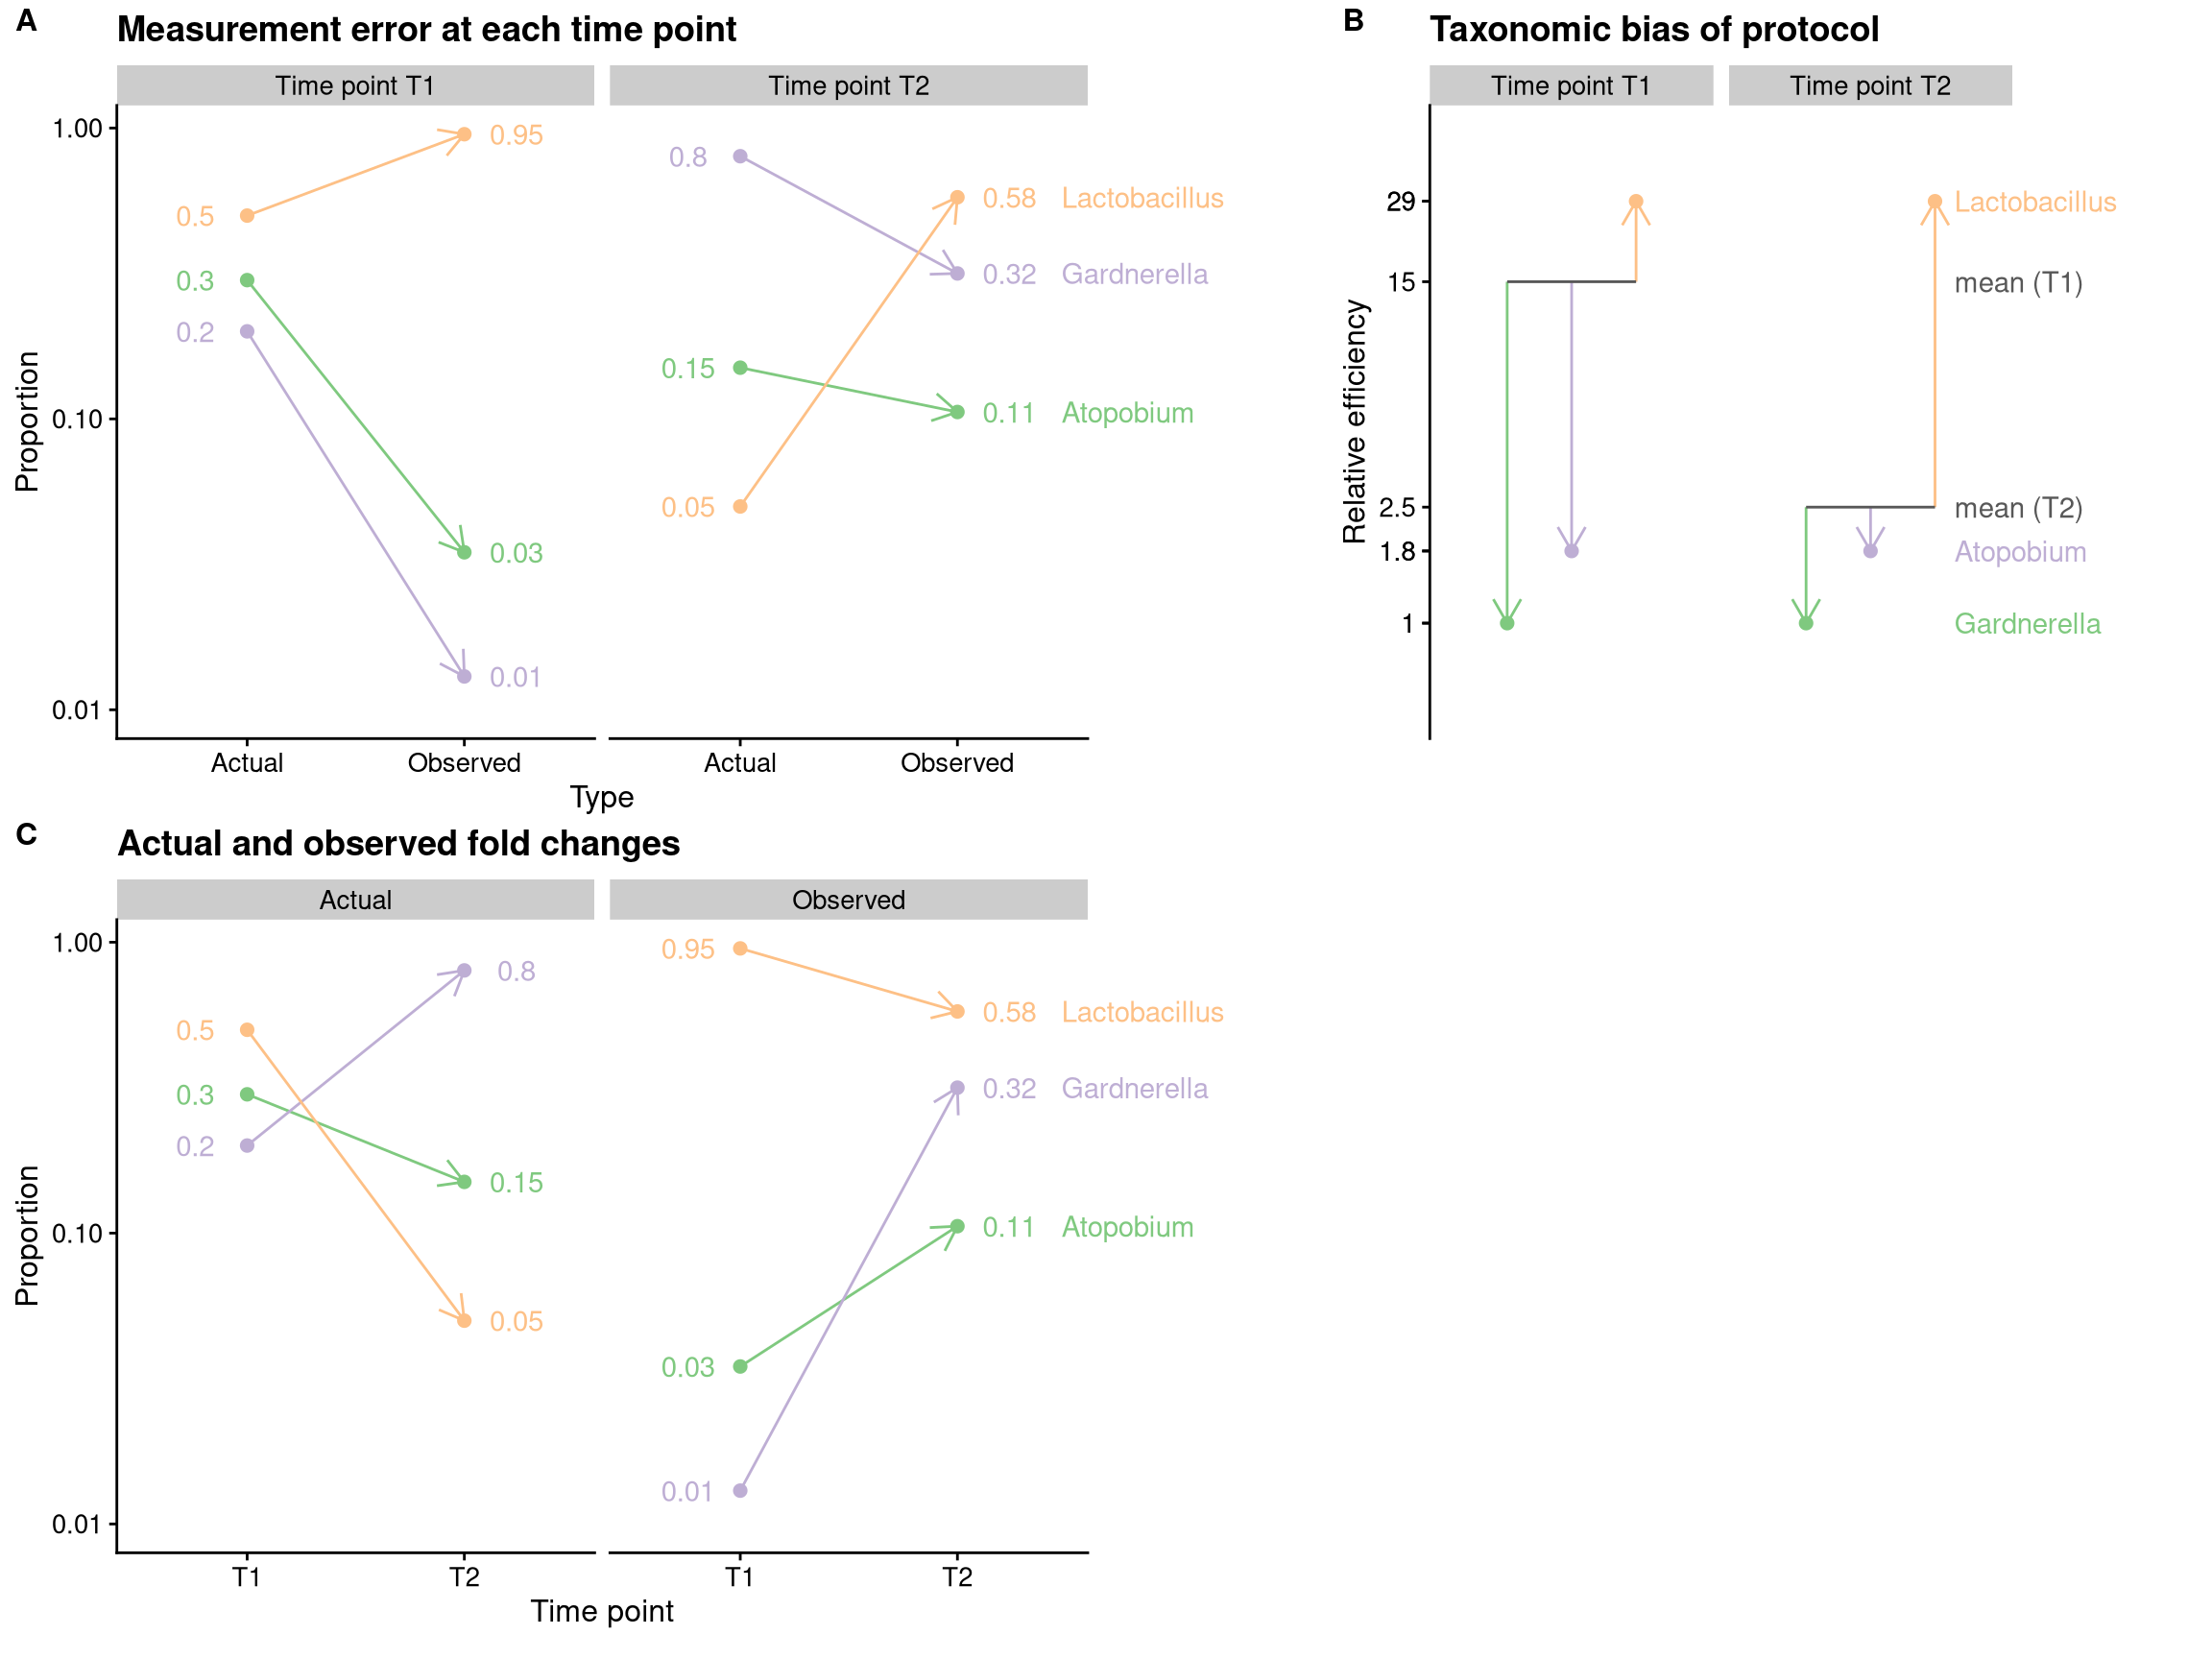
\includegraphics{_main_files/figure-latex/vaginal-example-1.pdf}
\caption{\label{fig:vaginal-example}\textbf{Taxonomic bias can distort differential abundance results even when it is consistent for each taxon across samples.} Panel A shows the actual and observed proportions for hypothetical community samples from two time points, which differ in their relative abundance of three taxa. Panel B shows taxonomic bias in terms of the relative efficiencies of the three taxa against the mean efficiency of each sample; the difference between the taxon's efficiency and the sample's mean (vertical arrows) determines the fold error seen in Panel A. Panel C rearranges the plot from Panel A to show the actual and observed fold changes between time points. The efficiencies of individual taxa were estimated by \protect\hyperlink{ref-mclaren2019cons}{McLaren, Willis, and Callahan} (\protect\hyperlink{ref-mclaren2019cons}{2019}) from mock community data from \protect\hyperlink{ref-brooks2015thet}{Brooks et al.} (\protect\hyperlink{ref-brooks2015thet}{2015}). The abundances are hypothetical but inspired by observations from the human vaginal microbiome; see main text.}
\end{figure}



We illustrate the problems posed by taxonomic bias for differential abundance using an example where the bias of an MGS protocol was explicitly measured using mock communities.
To analyze the effects of taxonomic bias on measurements of the human vaginal microbiome, \protect\hyperlink{ref-brooks2015thet}{Brooks et al.} (\protect\hyperlink{ref-brooks2015thet}{2015}) performed 16S rRNA gene sequencing of mock communities of seven key vaginal species using a similar protocol to that of the Vaginal Human Microbiome Project (VaHMP).
\protect\hyperlink{ref-mclaren2019cons}{McLaren, Willis, and Callahan} (\protect\hyperlink{ref-mclaren2019cons}{2019}) used this data to estimate the relative measurement efficiency of the seven species.
They found that the most efficiently measured species, \emph{Lactobacillus iners}, had an efficiency that was 29X that of the least efficiently measured species, \emph{Gardnerella vaginalis}, primarily due to a greater DNA extraction efficiency and 16S copy number.
A third species, \emph{Atopobium vaginae}, had an efficiency 1.8X that of \emph{G. vaginalis}.
A common aim of human vaginal microbiome studies, including the VaHMP, is to understand the causes and consequences of shifts in communities from being dominated by a particular \emph{Lactobacillus} species to dominance by a non-\emph{Lactobacillus} species such as \emph{G. vaginalis}, which have been associated with deleterious health outcomes including an increased risk of preterm births in pregnant women.
It is therefore important to know whether the efficiency variation found by \protect\hyperlink{ref-mclaren2019cons}{McLaren, Willis, and Callahan} (\protect\hyperlink{ref-mclaren2019cons}{2019}) affects the observed differential abundances between \emph{Lactobacillus}-dominated and \emph{Gardnerella}-dominated communities.

Figure \ref{fig:vaginal-example} illustrates the effects of taxonomic bias on the measured proportions for hypothetical vaginal samples from a single woman at two points in time, during which the community shifts from being dominated by \emph{Lactobacillus} to being dominated by \emph{Gardnerella}.
In each case, we observe a greater proportion of \emph{Lactobacillus} than is truly present, and less of the other two species (Figure \ref{fig:vaginal-example}A).
This positive multiplicative error arises because \emph{Lactobacillus} is more efficiently measured than the average species in each sample.
\protect\hyperlink{ref-mclaren2019cons}{McLaren, Willis, and Callahan} (\protect\hyperlink{ref-mclaren2019cons}{2019}) showed that the observed and actual proportions of a taxon \(i\) in a sample \(s\) are related by the equation
\begin{align}
  \label{eq:error}
  \text{observed}_{i}(s) = \text{actual}_{i}(s) \cdot \frac{\text{efficiency}_{i}}{\text{mean efficiency}(s)}
\end{align}
where \(\text{mean efficiency}(s)=\text{actual}_j(s)*\text{efficiency}_j\) in the denominator is the average efficiency of all taxa in that sample.
Intuitively, Equation \eqref{eq:error} says that the taxon will be overrepresented by the extent to which its measurement efficiency is greater than the average efficiency of cells in the sample.
Figure \ref{fig:vaginal-example}B shows the efficiencies of the three taxa and the mean efficiency in each sample.
The (multiplicative) difference between the taxon efficiencies and the mean efficiency determines the (multiplicative) error in each sample; for example, the mean efficiency in the second sample is 2.5, leading to a 29/2.5=11.6X error in the proportion of \emph{Lactobacillus}.
The error in the second sample is larger---specifically, by 6X---than the first sample because the high proportion of \emph{Gardnerella} has reduced the sample mean efficiency (and thus increased the efficiency of \emph{Lactobacillus} relative to the mean) by 6X.

The enrichment depends on the taxon's efficiency relative to the sample average, rather than the efficiency itself, because the requirement that the proportions of all taxa sum to one locks the taxa in a zero-sum competition.
Notably, competition occurs (though in a less absolute form) even at the level of the raw sequencing reads: DNA extractions and PCR reactions have limited output capacity; high-concentration samples are typically subsampled to fixed, lower concentrations; and sequencing libraries are given limited sequencing effort; so that the experimental process itself typically imposes competition to be sequenced.
And it is competition that prevents the effects of taxonomic bias from canceling when we analyze how the proportions of individual taxa change across samples.

Figure \ref{fig:vaginal-example}C shows the consequences of measurement error on an analysis of the fold change in proportions between the two samples.
In reality, \emph{Gardnerella} changes by 4X, \emph{Lactobacillus} by 0.1X, and \emph{Atopobium} by 0.5X.
Yet what is observed is that \emph{Gardnerella} changes by 32X, \emph{Lactobacillus} by 0.6X, and \emph{Atopobium} by 3X.
In other words, the change in each case is multiplied by 6X, causing a much larger increase in \emph{Gardnerella} and a smaller decrease \emph{Lactobacillus} than actual, and the appearance that \emph{Atopobium} increased when it in fact decreased.
Why do such errors occur?
The multiplicative error in Equation \eqref{eq:error} has two parts: a taxon-specific term in the numerator that is the same in each sample, and a taxon-independent term in the denominator that depends on the composition of the sample through the mean efficiency.
When we compute the fold change in a taxon i between samples s and t,
\begin{align}
  \frac{\text{observed}_{i}(t)}{\text{observed}_{i}(s)}=\frac{\text{actual}_{i}(t)}{\text{actual}_{i}(s)}*\frac{\text{efficiency}_{i}}{\text{efficiency}_{i}}*\frac{\text{mean efficiency}(s)}{\text{mean efficiency}(t)}
\end{align}
the constant efficiency in the numerator of Equation \eqref{eq:error} cancels, but the varying mean efficiency does not, leaving an error that is equal to the inverse change in mean efficiency.
As a result, we are here left inferring that the fold-changes in proportions have all increased less (or decreased more) than they truly have.
In our example, the mean efficiency decreased by 6X (from 15 to 2.5) due to the shift in dominant taxon from the high-efficiency \emph{Lactobacillus} to the low-efficiency \emph{Gardnerella}, causing the observed fold changes to increase by 6X above the actual.
This increase distorted the magnitudes of the changes in \emph{Lactobacillus} and \emph{Gardnerella} (decreasing the first and increasing the second) and changed the sign of \emph{Atopobium} from negative to positive.
Thus partial cancelling in the effect of a constant multiplicative bias may not be sufficient to protect against spurious results.

Spurious results can occur for the same basic reason in proportion-based absolute-abundance inference.
Suppose that the true total abundance in each sample can be determined experimentally.
Because the absolute abundance estimate simply multiplies the erroneous observed proportions by this total, the estimated change in absolute abundance is wrong by the same factor as the fold change in proportions.
In our Figure \ref{fig:vaginal-example} example, if the change in total abundance between samples were 2X, then we would observed both \emph{Lactobacillus} and \emph{Atopobium} to have increased in absolute abundance (by 1.2X and 6X), when in fact \emph{Lactobacillus} decreased (by 5X) and \emph{Atopobium} remained the same.

\hypertarget{effect-on-regression-of-multiple-samples}{%
\subsection{Effect on regression of multiple samples}\label{effect-on-regression-of-multiple-samples}}

We showed how fold changes of individual samples may be unreliable.
But microbiome analyses often do not interpret such individual differences, and instead look for average patterns across many samples, such as how the abundance of a taxon varies with some covariate of interest.
The covariate may be discrete, such as whether the sample is from a healthy or sick person, or it may be continuous, such as a measure of space, time, or temperature.
Often these analyses can be framed as a regression problem.
For example, we might hypothesize that the log absolute abundance of taxon \(i\) changes with a variable \(x\) according to the simple linear regression,
\begin{align}
  E[\text{log abundance}_{i} \mid x] = a_{0} + a_{1}x
\end{align}
where \(x\) is either continuous (e.g., sediment depth) or binary (e.g., \(x=1\) for treated patients and \(x=0\) for controls).
Much of the effect of bias will be absorbed by the model intercept, which is typically not of interest to the researcher.
However, variation in the mean efficiency creates additional variation (reducing statistical power to detect variation in the slope) and can also create a statistical bias in our slope estimate equal to the inverse slope of \(E[\text{log mean efficiency}\mid x]\) as a function of \(x\).
Therefore if the mean efficiency varies across samples, but is not associated with the covariate \(x\), its effect may simply be to create larger standard errors in our slope estimate.
But the larger worry may be the systematically distorted slope (\(a_1\)) estimates that arise in situations where the mean efficiency changes with \(x\).
Notably, the error in an absolute sense is the same for all taxa---the slope is always reduced by the same amount---but the implications differ for various taxa depending on their slopes, causing magnitude or sign errors depending how the coefficient derived from the (unknown) true abundances compares to that of the mean efficiency (Figure \ref{fig:regression-example}).

\begin{verbatim}
#> Warning: Package `magick` is required to draw images. Image not drawn.
\end{verbatim}

\begin{figure}
\centering
\includegraphics{_main_files/figure-latex/regression-example-1.pdf}
\caption{\label{fig:regression-example}\textbf{Taxonomic bias distorts multi-sample differential abundance inference when the mean efficiency of samples is associated with the covariate of interest.} Details to synthesize into a caption: Regression of log2(Proportion) of the commensal fungus Penicillium versus timepoint; timepoints 1 and 2 are pre- and post-challenge with the pathogen Melampsora. Data is split by the region the host plants are derived from (Eastern and Western US). Calibrated proportions = Observed proportions in the real, experimental samples after adjustment for the bias measured in mock communities. Mean efficiency of each community is inferred by treating the calibrated proportions as the truth, and multiplying by efficiencies estimated from the mocks. The pathogen Melampsora has a high measurement efficiency; thus once it infects the plants, the mean efficiency of the sample increases (purple points). Efficiency is here taken as relative to the focal taxon Penicillium. West plants tend to be more resistant to the pathogen, which likely explains why the mean efficiency doesn't increase as much in the West plants. Penicillium is observed to decrease in log proportion, in both the East and West plants. But the calibrated measurements show that it actually slightly increases in the East plants, and has a lesser decrease in the West plants than what was observed before bias correction. The difference between the Calibrated and Observed data points and regression lines equals the regression line of the mean efficiency: Orange = Green + Purple; Green = Orange - Purple. The absolute error in regression coefficients is the same for all taxa. I picked Penicillium for illustration since it has the smallest observed decrease, which makes the error due to bias have a particularly significant impact.}
\end{figure}



\hypertarget{implications-for-real-world-inference}{%
\section{Implications for real-world inference~}\label{implications-for-real-world-inference}}

These observations show that the effects of taxonomic bias do in fact cause error in proportion-based differential abundance analyses.
Yet if the mean efficiency varies much less across samples than the abundances of individual taxa, this error will be negligible.
Alternatively, if variation in the mean efficiency is effectively random (not associated with regression covariates), the effect of bias may be to increase the residual variance and thus reduce our statistical power to assay differential abundance---unfortunate to be sure, but perhaps not as much as confidently inferring changes with the wrong sign or magnitude.
But there are salient biological scenarios where substantial associations between the mean efficiency and covariate can in fact lead to spurious differential abundance inference.

\hypertarget{scenarios-in-which-bias-may-cause-spurious-results}{%
\subsection{Scenarios in which bias may cause spurious results}\label{scenarios-in-which-bias-may-cause-spurious-results}}

Figure \ref{fig:vaginal-example} illustrates how a change in dominance by from a high- to low- efficiency taxon (or vice versa) can easily create spurious DA results.
Indeed, this scenario may be particularly common in vaginal microbiome studies.
Human microbiomes often dominated by \emph{Lactobacillus}, but can become dominated by non-\emph{Lactobacillus} species such as \emph{Gardnerella} vaginalis and \emph{Atopobium vaginae}, and these low-\emph{Lactobacillus} states are associated with the disease bacterial vaginosis and, in pregnant women, an increased risk of preterm birth.
Using mock community measurements from \protect\hyperlink{ref-brooks2015thet}{Brooks et al.} (\protect\hyperlink{ref-brooks2015thet}{2015}), \protect\hyperlink{ref-mclaren2019cons}{McLaren, Willis, and Callahan} (\protect\hyperlink{ref-mclaren2019cons}{2019}) showed that the efficiency of two common \emph{Lactobacillus} species were 20-30X greater than \emph{G. vaginalis} and \emph{A. vaginae}.
Therefore we should expect samples dominated by \emph{Lactobacillus} to have a much larger mean efficiency than those those dominated by \emph{G. vaginalis} and \emph{A. vaginae}, which would distort the observed associations of all taxa with any covariate that is also associated with \emph{Lactobacillus} dominance.
The extraction and 16S sequencing protocol used by \protect\hyperlink{ref-brooks2015thet}{Brooks et al.} (\protect\hyperlink{ref-brooks2015thet}{2015}) is similar to that used in the VaHMP MOMs-PI study also led by these researchers to investigate the associations of these taxa with preterm birth (\protect\hyperlink{ref-fettweis2019thev}{Fettweis et al.} (\protect\hyperlink{ref-fettweis2019thev}{2019})), demonstrating the potential for serious real-world consequences for these statistical/technical concerns.

Similar dynamics occur in a plant-fungal interactions experiment performed by \protect\hyperlink{ref-leopold2020host}{Leopold and Busby} (\protect\hyperlink{ref-leopold2020host}{2020}) (Figure \ref{fig:regression-example}).
The authors inoculated commensally-colonized trees with a fungal pathogen.
Using DNA mock communities, they showed that (excluding bias from DNA extraction) the pathogen was 10X more efficiently measured than the median commensal and 40X more efficiently measured than the lowest-efficiency commensal.
In most hosts, the pathogen increased rapidly between timepoints, driving an increase in the sample mean efficiency that in turn leads to larger decreases being observed in the proportions of commensal taxa than what is predicted using calibrated (bias-corrected) values (REF APPENDIX).
For example, the calibrated proportions indicate that the commensal \emph{Penicillium} slightly increased in hosts from the Eastern US and slightly decreased in hosts from the Western US.
Yet the observed (uncalibrated) proportions show moderate and large decreases, respectively (Figure \ref{fig:regression-example} above).

These examples involved scenarios where individual taxa can constitute a large proportion of the community.
But in samples from highly-diverse ecosystems such as human gut, soil, and ocean sediment, one species rarely dominates.
In these cases it might seem intuitive that the mean efficiency should be relatively stable across samples: As diversity increases, the mean efficiency effectively averages over efficiencies from a greater number of taxa and so (by the central limit theorem) will converge to a constant value---if taxon efficiencies are statistically independent of taxon abundances (REF APPENDIX).
In practice, associations between efficiencies and abundances may be common and can allow large shifts in mean efficiency to occur even in highly diverse samples.

The human gut provides a clear example of how such associations might arise.
Gut microbiomes typically have high diversity at the species level but are dominated by just a small number of phyla, and two in particular: The Bacteroidetes and the Firmicutes.
The ratio of Bacteroidetes to Firmicutes can shift substantially between individuals and has been linked to a number of host traits and health conditions.
In addition, many DNA extraction protocols more efficiently lyse Gram-negative Bacteroidetes species than Gram-positive Firmicutes species (though there can also be significant variation in extraction efficiency among species within these phyla (\protect\hyperlink{ref-mclaren2019cons}{McLaren, Willis, and Callahan} (\protect\hyperlink{ref-mclaren2019cons}{2019})).
For such protocols, we should expect Bacteroidetes-dominated samples to have substantially larger mean efficiencies than Firmicutes-dominated samples, regardless of species-level diversity.
This association of efficiency with phylum abundance will distort DA inferences at any taxonomic level if the covariate is also associated with these phyla.

This example illustrates a general mechanism by which association between the abundances and efficiencies of taxa are created by the common influence of evolutionary history.
Just as shared evolutionary history creates positive associations in ecological traits that drives positive correlations in how related taxa vary in abundance across samples, so does it create positive associations in bias-related traits that can lead to similar efficiencies among closely related taxa.
Such phylogenically-associated, bias-affecting traits include cell-wall toughness, ribosomal-operon copy number, binding affinity for a given set of primers, and representativeness in taxonomic databases.
Ecology and efficiency are both affected by the same evolutionary history, leading to positive associations between the two: A change in diet that increases the relative abundances of many Bacteroidetes species and in so doing also increases the relative abundance of many easy-to-lyse species.

Associations between measurement efficiency and relative abundance can also arise because a single trait affects both.
For example, microbes at the ocean floor are slowly buried, sinking into a low nutrient, low oxygen environment.
\protect\hyperlink{ref-lloyd2020evid}{Lloyd et al.} (\protect\hyperlink{ref-lloyd2020evid}{2020}) estimate the log fold change in the estimated absolute abundance of various taxa with sediment depth (as a proxy for time) to determine which taxa are able to persist and even grow in this difficult environment.
It is plausible that microbes with tougher cell walls would tend to persist longer (alive or dead) in the sediment, while at the same time being more difficult to extract DNA from than microbes with weaker cell walls.
As the relative abundance of tougher species increases with depth, the mean extraction efficiency decreases.
This decrease would increase the inferred log fold changes and could lead to inferred growth of taxa that are actually just persisting or even slowly dying off.
Another example of a trait that might simultaneously affect efficiency and relative abundance is ribosomal copy number, which increases the measurement efficiency in ribosomal amplicon experiments and is also linked to differences in ecology and population dynamics among species.

\hypertarget{error-in-absolute-abundance-measurements}{%
\subsubsection{Error in absolute abundance measurements}\label{error-in-absolute-abundance-measurements}}

So far we have ignored error associated with our absolute abundance measurements.
In fact, these measurements can also have a tendency to measure contributions from some taxa more efficiently than others.
\textbf{TODO: State how this could create problems.
Might also note the ambiguity in what the truth/target is (e.g.
live cells, or all cells; cells, or 16S rRNA gene copies; observations in Jian, Salonen, and Korpela 2021).}
Interestingly, taxonomic bias may actually make qPCR a better method for absolute quantification than cell counting for 16S rRNA gene sequencing experiments.
16S rRNA gene qPCR measures the concentration of 16S rRNA gene copies in the extracted DNA and is therefore necessarily affected by three large sources of bias in 16S rRNA gene experiments: extraction, amplification, and copy-number variation.
Yet these biases are shared by the sequencing measurement.
Though they make qPCR measurements a bad proxy for total cell density, when used for absolute differential abundance inference the shared bias in the qPCR and sequencing measurements can cancel, leaving relative accurate fold changes.
(Jian, Salonen, and Korpela 2021 suggests some of these ideas and APPENDIX gives a mathematical justification.)
If common primers are used by qPCR and 16S rRNA gene sequencing, the bias due to primer mismatches and other sources of variation in amplification could even be accounted for in this manner.
Yet ideally we would still be able to estimate and correct remaining error due to unshared bias or to mechanisms, such as saturation during DNA extraction, that could break the assumed proportionality between qPCR measurements and total abundance.

\hypertarget{we-cannot-simply-ignore-taxonomic-bias}{%
\subsection{We cannot simply ignore taxonomic bias}\label{we-cannot-simply-ignore-taxonomic-bias}}

These examples show that there is potential for bias to distort DA results in both low and high diversity settings.
We therefore need methods to control or correct for bias to ensure the validity of future results, as well as methods to probe the robustness of past results.
It is possible that spurious results are unlikely in many experimental contexts.
By applying such methods across a range of biological and experimental contexts we will deepen our understanding of when bias is unlikely to significantly distort biological findings and when additional measures are needed to mitigate its effects.

\hypertarget{potential-solutions}{%
\section{Potential solutions}\label{potential-solutions}}

\hypertarget{using-control-samples-to-calibrate-relative-abundances}{%
\subsection{Using control samples to calibrate relative abundances}\label{using-control-samples-to-calibrate-relative-abundances}}

In principle, control (``mock'') communities containing representative taxa from the environment of interest can be used to directly estimate the measurement efficiencies and correct bias in the MGS measurements (``calibration'').
Such an approach may be sufficient for synthetic-community experiments, where all taxa are culturable, and for relatively simple natural communities like the vaginal microbiome that are dominated by a small number of culturable taxa.
But suitable mock controls may not be feasible for most complex natural ecosystems and require significant effort to develop.

An closely-related alternative to mocks are controls derivedd from natural samples, which provide a way to calibrate measurements from protocols to a reference protocol (\protect\hyperlink{ref-mclaren2019cons}{McLaren, Willis, and Callahan} (\protect\hyperlink{ref-mclaren2019cons}{2019})).
A natural fecal standard is currently being developed by \href{https://www.nist.gov/programs-projects/human-gut-microbiome-reference-material}{NIST} and one has recently been made available commercially by Zymo Research (\href{https://www.zymoresearch.com/collections/zymobiomics-microbial-community-standards/products/zymobiomics-fecal-reference-with-trumatrix-technology}{ZymoBIOMICS Fecal Reference}).
Ensuring the stability and homogeneity of such control samples can be challenging.
Careful testing is also needed to ensure that the preparation and storage of the controls has not significantly affected the taxonomic bias relative to the experimental samples in a given application.
As it is feasible to characterize a single standard much more extensively than a typical community sample, we may be able to obtain an estimated composition we feel comfortable treating as the ground truth.
Yet even when this is not possible, such natural standards can allow us to reconcile results across studies despite not knowing the truth.

\hypertarget{ratio-based-relative-and-absolute-abundance-inference}{%
\subsection{Ratio-based relative and absolute abundance inference}\label{ratio-based-relative-and-absolute-abundance-inference}}

A comprehensive approach of estimating the efficiency of all taxa is needed for getting calibrated relative abundances of all taxa within individual samples.
But what if we only want calibrated DA analysis?
That is, we are comfortable with not knowing whether \emph{E. coli} is 10\% of our sample if we can confidently determine that it doubled or halved between sample conditions?
This problem is easier to solve, and one solution is to use analysis methods based on the ratios among taxa rather than the proportions of individual taxa.

A subset of methods for analyzing differential relative abundance are derived from the field of Compositional Data Analysis (CoDA).
The defining feature of CoDA methods is that they are based on fold-changes in ratios among elements (here, the taxa) (REF AITCHISON).
The use of CoDA methods in microbiome analysis has largely been motivated by concerns over the negative correlations between taxa induced by the sum-to-one constraint in taxon proportions.
But \protect\hyperlink{ref-mclaren2019cons}{McLaren, Willis, and Callahan} (\protect\hyperlink{ref-mclaren2019cons}{2019}) showed that, due to their property of perturbation invariance (REF AITCHISON), the results of CoDA differential relative abundance analysis are invariant to consistent taxonomic bias.
From Equation \eqref{eq:error}, the observed ratio of a taxon \(i\) to a taxon \(j\) in a sample \(s\) is
\begin{align}
  \frac{\text{observed}_{i}}{\text{observed}_{j}}=\frac{\text{actual}_{i}}{\text{actual}_{j}}*\frac{\text{efficiency}_{i}}{\text{efficiency}_{j}}
\end{align}
The error is independent of the sample composition and thus cancels in any function that is a fold-change of this (or any) ratio of taxa between samples.
(Perhaps insert example from Figure \ref{fig:vaginal-example}ABC all giving same ratio FCs.)

Might ratio-based analysis also be used to overcome the effects of bias in differential absolute abundance?
In fact, some methods for determining absolute abundance are based on ratios among taxa in the MGS measurement instead of proportions.
Rather than using a measurement of total abundance, these methods require determining the abundance of one or more reference taxa.
To estimate the abundance of a focal taxon \(i\), this approach multiplies the ratio of reads (or proportions) of taxon i to a reference taxon \(r\) by a known or estimated abundance of the reference taxon, (while ignoring bias)
\begin{align}
  \text{estimate}_{i} = \frac{\text{observed}_{i}}{\text{observed}_{r}}*\text{abundance}_{r}
\end{align}
So far this approach has been mainly used with spike-in experiments, in which an extraneous taxon is added in a known (and typically constant) abundance to each sample so that it can serve as the reference taxon.
Yet the reference taxon could also be a naturally occurring taxon whose absolute abundance we have estimated using a method such as ddPCR directly on cells or (q/dd)PCR on the extracted DNA.
Because taxa do not compete (or competition is greatly reduced) in such targeted measurements, any taxonomic bias associated with them is expected to create constant multiplicative error across samples and so not affect fold change estimates {[}APPENDIX{]}.
APPENDIX describe various theoretical and experimental considerations for both approaches.

\hypertarget{estimating-error-with-targeted-measurements-of-a-small-number-of-taxa}{%
\subsection{Estimating error with targeted measurements of a small number of taxa}\label{estimating-error-with-targeted-measurements-of-a-small-number-of-taxa}}

Because targeted absolute-abundance measurements are expected to provide (relatively) accurate estimates of fold changes, they can be used to validate and even correct the DA results derived from a proportion-based absolute DA analysis.
We illustrate the basic idea using the \protect\hyperlink{ref-lloyd2020evid}{Lloyd et al.} (\protect\hyperlink{ref-lloyd2020evid}{2020}) experiment described above.
Absolute abundances in this study were estimated by multiplying MGS proportions by total abundance measured by cell counting; for comparison, qPCR was used to measure specific microbial taxa.
Because the error in fold changes or a regression from the MGS measurements is taxon-independent, the difference between the two methods for these reference taxa informs us about the difference for all taxa.
\protect\hyperlink{ref-lloyd2020evid}{Lloyd et al.} (\protect\hyperlink{ref-lloyd2020evid}{2020}) found close agreement for the specific taxa also measured by qPCR (Table 1), suggesting that variation in sample mean efficiency did not significantly distort their results.
In principle, a joint statistical analysis of all measurements would allow inferring variation in the sample mean efficiency across samples and obtaining calibrated fold change and regression estimates for all taxa {[}APPENDIX{]}.

\hypertarget{computational-approaches}{%
\subsection{Computational approaches}\label{computational-approaches}}

What can we do for experiments that have already been conducted without mock controls, targeted control measurements, or spike-ins?
At least two purely computational approaches can still be used.

\textbf{Bias sensitivity analysis:}
A straightforward and universally available approach is to use computer simulation to determine how the results change under a range of possible sets of efficiencies, which can be randomly generated to reflect certain hypotheses about bias in the given system.
The utility of such simulations can increase the more we learn about the magnitude of bias in different systems and the taxonomic and protocol features that determine it.
Future work in developing tools and methods for simulating efficiency vectors and performing bias sensitivity analyses could be a valuable way to assay and improve the reliability of microbiome results---not just for differential absolute abundance, but for all microbiome analyses.

\textbf{Bias-aware meta-analysis:}
When the goal is to perform a meta-analysis that combines studies that have used different protocols, the unknown measurement efficiencies of each protocol can be explicitly included as parameters of the statistical model that is used.
Unknown efficiencies can be included in ``compositional'' linear modeling frameworks such as ALDEx2, DivNet, and fido simply by adding a protocol-specific term to the linear model of taxon log ratios.
Thus such bias-aware meta-analyses are already technically feasible and---if bias is truly consistent within a protocol or study---may provide a more powerful alternative to non-parametric or other meta-analysis methods that do not explicitly model bias.

\hypertarget{appendix-appendix}{%
\appendix \addcontentsline{toc}{section}{\appendixname}}


\hypertarget{models}{%
\section{Measurement models}\label{models}}

Deterministic measurement error models that extends the \protect\hyperlink{ref-mclaren2019cons}{McLaren, Willis, and Callahan} (\protect\hyperlink{ref-mclaren2019cons}{2019}) model of metagenomics measurement to 1) describe absolute as well as relative abundance, 2) include spike-in taxa, and 3) include supplementary measurements of bulk and targeted (absolute) abundance.

\hypertarget{actual-abundances-and-general-notation}{%
\subsection{Actual abundances and general notation}\label{actual-abundances-and-general-notation}}

(For now) Number of samples = J; Number of taxa = I.

\(A_{ij}\) is the actual absolute abundance of taxon \(i\) in sample \(j\), in the target units.
For variables that hold matrixes or vectors, capital letters denote absolute abundances and lower case letters denote proportions.
Thus \(a_{ij}\) is the matrix of actual relative abundances in terms of cells as a proportion of the total amount of cells in the sample; \(a_{ij} = A_{ij} / A_{Tj}\).
Let \(A_{Tj}\) (or \(A_{\cdot j}\)??) be the total abundance in sample \(j\), \(A_{Tj} = \sum_i A_{ij}\).
For a subset of taxa \(Q \subset \{1, \dots, I\}\), define \(A_{Qj} \equiv \sum_{i \in Q} A_{ij}\) to be the total abundance of the taxa in \(Q\).

Unless specified otherwise, \(A\) always refers to abundance in the original sample material, not in extracted DNA.
I will assume the target units are concentration of cells per unit mass. However, other units (such as biomass per volume) may be relevant.

To consider various addition information that can be used for absolute abundance inference, I let \(B\) denote bulk abundance measurements (such as via flow cytometry or broad-range 16S qPCR), \(S\) denote the known taxon abundances of a spike-in, and \(T\) denote the abundances of a set of taxa made via targeted measurement.
I let \(R \subset \{1, \dots, I\}\) denote the set of \emph{reference taxa} whose abundance is known independently from the metagenomics measurement (up to experimental bias factors) because they were spiked at a known density, subjected to a targeted measurement, or have been determined through some other means to have a constant or known abundance across samples.

Bias vectors \(B^{(P)}\) are vectors of length \(I\) indicating the taxon-specific bias associated with a measurement protocol \(P\).
I generally assume these to be sample-independent.
An overbar denotes the average value over taxa weighted by actual abundance; i.e., \(\bar B_j = I^{-1} \sum_i B_i a_{ij}\).
An overbar and a subcript set of taxa indicates the mean bias within that subset: \(\bar B_{Qj} = \sum_{i\in Q} B_i a_{ij} / \sum_{i\in Q} a_{ij}\).

\begin{longtable}[]{@{}llll@{}}
\toprule
Measurement type & Units & Abundance matrix & Bias vector \\
\midrule
\endhead
\textbf{A}ctual abundance & {[}cells{]} & \(A\), \(a\) (\(I\times J\)) & - \\
\textbf{M}etagenomics & counts & \(M\), \(m\) (\(I\times J\)) & \(B^{(M)}\) \\
Bul\textbf{k} abundance & {[}cells{]}, {[}DNA{]}, or {[}gene copies{]} & \(K\) (\(I\times 1\) column vector) & \(B^{(K)}\) \\
\textbf{T}argeted abundance & {[}cells{]}, {[}DNA{]}, or {[}gene copies{]} & \(T\) (\(I \times J\)) & \(B^{(T)}\) \\
\textbf{S}pike-in abundance & {[}cells{]}, {[}DNA{]}, or {[}gene copies{]} & \(S\) (\(I \times J\)) & \(B^{(S)}\) \\
\bottomrule
\end{longtable}

Note: \(S_{ij}\) and \(T_{ij}\) are only defined for the reference taxa \(i \in R\).

\hypertarget{metagenomics-measurement}{%
\subsection{Metagenomics measurement}\label{metagenomics-measurement}}

\(M\) is an \(I\times J\) matrix representing the (marker-gene or) metagenomics measurement; \(M_{ij}\) is the sequencing count associated with taxon \(i\) in sample \(j\), such that \(M_{ij} = 10\) indicates that 10 fragments of DNA were sequenced and assigned to taxon \(i\) and sample \(j\).
In the case of paired-end sequencing, a single fragment of DNA yields two reads, which may or may not be counted jointly or independently by different algorithms; here I assume that read-pairs are assigned jointly, and will use ``read'' and ``fragment'' interchangeably.
For simplicity, I ignore the possibility for index switching or other sources of cross-contamination and assume that reads assigned to sample \(j\) truly arose from sample \(j\).

Following the notation defined above, I let \(M_{Tj} = \sum_i M_{ij}\) be the total count for sample \(j\); I will sometimes refer to this number as the \emph{sequencing depth} or \emph{read depth} of the sample, though in reality the total count will be less than the sample's sequencing depth since often a significant fraction of reads are lost by filtering steps prior to producing the final count matrix.
I use \(m_{ij} = M_{ij} / M_{Tj}\) to denote the proportion of reads assigned to taxon \(i\) in sample \(j\).

I assume that the composition (relative abundances) is given by the deterministic error model presented in \protect\hyperlink{ref-mclaren2019cons}{McLaren, Willis, and Callahan} (\protect\hyperlink{ref-mclaren2019cons}{2019}).
In this model, the bias vector \(B^{(M)}\) represents the \emph{relative} efficiencies with which various taxa are measured, and so has the same effect on measurement if we rescale it \(B \to cB\) for any \(c > 0\).
To remove this degree of freedom, I will suppose that \(B^{(M)}_{1} = 1\), so that \(B^{(M)}_i\) is the efficiency of taxon \(i\) relative to the first taxon.
We may take the definition of the MWC model as being that, conditional on the total count \(M_{Tj}\), the observed read count of taxon \(i\) is proportional to its actual abundance times its efficiency times a taxon-independent factor \(C_j\) chosen to make sample \(j\)'s counts sum to \(M_{Tj}\),
\begin{align}
  \label{eq:M}
  M_{ij} = A_{ij} B^{(M)}_{i} C_j, && 
  C_j = \frac{M_{Tj}}{\sum_i A_{ij} B^{(M)}_{i}}
      = \frac{M_{Tj}}{A_{Tj} \bar B^{(M)}_j}.
\end{align}
In this model, the ratios among taxa are distorted by constant factors; for two taxa \(i\) and \(i'\),
\begin{align}
  \label{eq:M-ratio}
  \frac{M_{ij}}{M_{i'j}} 
    = \frac{m_{ij}}{m_{i'j}} 
    = \frac{A_{ij}}{A_{i'j}} \cdot \frac{B^{(M)}_{i}}{B^{(M)}_{i'}}
\end{align}
for all samples \(j\).
If one or both taxa are absent (\(A_i = 0\)) or undetectable (\(B_i = 0\)), both sides of the equation are either \(0\), \(\infty\), or \(0/0\) (undefined).
The observed proportion of a taxon equals its actual proportion multiplied by its efficiency relative to the sample mean efficiency,
\begin{align}
  \label{eq:m}
  m_{ij} = a_{ij} \cdot \frac{B_i}{\bar B^{(M)}_j}.
\end{align}

\hypertarget{bulk-absolute-abundance-measurement}{%
\subsection{Bulk absolute abundance measurement}\label{bulk-absolute-abundance-measurement}}

Consider estimating the total absolute abundance \(A_{T}\) via an aggregate or broad-range measurement, such as cell counting, flow cytometry, universal 16S qPCR, or total DNA concentration (e.g.~Qubit).
I let \(K_j\) donote the bulk absolute abundance measurement for sample \(j\) (mneumonic: ``K'' for the last letter in ``bulk'').

Bulk measurements are affected by taxon-specific bias \(B^{(K)}\), where \(B^{(K)}_i\) indicates how efficiently cells of taxon \(i\) contribute to the bulk measurement \(K\).
Unlike the metagenomics efficiencies, these bulk measurement efficiencies are absolute numbers.
For example, cells of one taxon may be more reliably counted than another; and for broad-range 16S qPCR measurement, we expect taxa to contribute in proportion to how reliably they are lysed and to their 16S copy number.
Let \(B^{(K)}_i\) denote the absolute efficiency with which a cell of taxon \(i\) contributes to the measurement in sample \(s\), which I assume is sample-independent.
We can write the estimate as
\begin{align}
  \label{eq:K}
  K_j = \sum_i A_{ij} B^{(K)}_i = A_{Tj} \bar B^{(K)}_j,
\end{align}
where \(\bar B^{(K)}_j\) is the mean bulk-measurement efficiency in the sample.

\hypertarget{targeted-absolute-abundance-measurement}{%
\subsection{Targeted absolute abundance measurement}\label{targeted-absolute-abundance-measurement}}

Targeted measurement of the absolute abundance of specific taxa can be made via a method such as qPCR, ddPCR, or counting CFUs selective media.
These measurements too may be subject to bias;
I suppose that the measurement of taxon \(i\) is given by
\begin{align}
  \label{eq:T}
  T_{ij} = A_{ij} B^{(T)}_i,
\end{align}
where \(B^{(T)}_i\) is the sample-independent, taxon-specific efficiency of the targeted measurement for taxon \(i\).

In discussing the case of multiple reference taxa, it will be useful to refer to the total targeted and metagenomics abundance and the average targeted and metagenomics efficiencies of the reference taxa.
I do so with the notation \(A_{Rj}\) and \(M_{Rj}\) (total abundances) and \(\bar B^{(T)}_{Rj}\) and \(\bar B^{(M)}_{Rj}\) (mean efficiencies) as defined above.
Note that
\begin{align}
  \label{eq:T-Rj}
  T_{Rj} 
    &= A_{Rj} \cdot \sum_{r \in R} \frac{A_{rj}}{A_{Rj}} \bar B^{(T)}_{Rj}
  \\&= A_{Rj} \bar B^{(T)}_{Rj}.
\end{align}

\hypertarget{spike-ins}{%
\subsection{Spike-ins}\label{spike-ins}}

The matrix \(S\) describes the nominal abundances with which spike-in taxa were added to each sample.
Spike-in experiments are often designed so that a taxon \(i\) is added in the same concentration to all samples, which we can represent by supposing the defined columns of \(S\) to be identical.
The bias \(B^{(S)}\) should be interpreted as error in the quantification of how much spike-in was added, such that
\begin{align}
  \label{eq:S}
  S_{ij} = A_{ij} B^{(S)}_i.
\end{align}
I assume that this error is constant across samples.
The motivation for this error model is as follows: Suppose that we misestimated the proportion of spike-in taxon \(s\in I_S\) in our original spike-in stock, by a factor \(B^{(S)}_s\); now its true abundance will be off by that factor in any spike-in derived from the starting stock.
Unlike the metagenomics efficiencies, these error factors are absolute numbers.

Taxa can be added as cells (pre-extraction) or as DNA (post-extraction).
In an application where DNA spike-ins are used to make inferences about changes in absolute cell abundances, we can include the difference between the nominal abundances \(S\) (the spiked DNA concentration) and the actual abundances \(A\) that are expected due to factors such as DNA extraction and copy-number variation in the bias term \(B^{(S)}\), so long as DNA extraction is linear (see section on saturation effects below).

(If we want to allow for different targeted and spike-in taxa, we can use \(R_S\) and \(R_T\).)

\hypertarget{complications}{%
\subsection{Complications}\label{complications}}

These models are the simplest for these types of experiments that have taxon-specific bias.
They therefore are idealizations that may be violated by real experiments in ways that affect our conclusions.
Here I list some relevant complications that we will return to in our analysis.
For more considerations, see the Discussion of \protect\hyperlink{ref-mclaren2019cons}{McLaren, Willis, and Callahan} (\protect\hyperlink{ref-mclaren2019cons}{2019}).

\hypertarget{abundances-units-and-protocol-stages}{%
\subsubsection{Abundances units and protocol stages}\label{abundances-units-and-protocol-stages}}

\emph{Still need to find the right way to synthesize these issues.}

qPCR measurements directly estimating the concentration of a marker gene in the extracted DNA.
Efficiency factors can translate the units from DNA to cell concentration \emph{and} account for the bias imposed by extraction and marker-gene CNV (copy-number variation).
Sometimes we may want to refer to the DNA concentrations in the sample after extraction, and in that case I will use the variable \(D\), and (perhaps) use \(B^{(T/D)}\) to refer to the bias of the targeted measurement vs the DNA concentrations it was applied to.
This can be useful when we are considering qPCR and also DNA spike-ins.

Note that the ``actual'' units could be chosen by the researcher to be something other than cell density; e.g.~biomass, or even 16S density.
But for concreteness I'll take to be cell density, as this seems to be what is most typically meant.

\hypertarget{saturation-in-dna-extraction-yields}{%
\subsubsection{Saturation in DNA extraction yields}\label{saturation-in-dna-extraction-yields}}

The equation for bulk measurement reflects an idealized form of bulk measurement in which, for a fixed taxonomic composition, \(K_j\) is directly proportional to \(A_T\).
However, a more realistic model for qPCR may be that \(K_j\) is a saturating function of \(A_T\), due to factors such as enzyme consumption or saturation in the elution step creating saturation in DNA yield during extraction.
However, it is not clear what this function should depend on (input biomass, cell concentration, total DNA?) and it is not clear what bias components should be included in determining the saturation, and these are not simply \(\bar B\) since that includes 16S copy-number which isn't relevant here.
Rather than try to accurately model the relationship between \(K\) and \(A\) in this more complicated scenario, I will use the models \(K_j = f(A_{Tj})\) and/or \(K_j = f(A_{Tj}\bar B^{(K)}_j)\) to get some intuition for the effect that a strong saturation effect has on our inferences when it is not accounted for.

Saturation during extraction also implications for targeted PCR measurements but not for measurements that work directly on cells; and for DNA spike-ins, but not cellular spike-ins.

\hypertarget{taxonomic-resolution-of-measurements}{%
\subsubsection{Taxonomic resolution of measurements}\label{taxonomic-resolution-of-measurements}}

I suppose that the ``taxa'' we consider are well-defined in a special sense, such that they can be equated both across samples within a measurement type and across different measurement types.
In other words, I assume that there is a real group of organisms corresponding to ``taxon \(i\)'' with abundance \(A_{i\cdot}\) that the various ``taxon \(i\)'' measurements are really measuring, such that we can, for example, directly equate the taxonomic source of the counts \(M_{i\cdot}\) and the targeted measurement \(T_{i\cdot}\).
Achieving this situation in practice requires careful attention to things like primer design and how the metagenomic taxonomic assignment is done, and even then it may not always be possible.

One important special case where this assumption breaks down is when measurements aggregate one or more of the \emph{atomic taxa} (corresponding to the rows in \(A\)), possibly in different ways by different measurement types.
This raises at least two sorts of complications.
First, constant multplicative bias at the level of atomic taxa does not translate into constant bias at the level of aggregate taxa (\protect\hyperlink{ref-mclaren2019cons}{McLaren, Willis, and Callahan 2019}).
Second, measurements may target different aggregates.
For example, if our metagenomics protocol provides ASV or species-level estimates but our PCR-based targeted measurements may quantify a genus or family.
Often through sufficiently careful bioinformatics we can at least nest the metagenomics taxa within the targeted taxon, but complications remain if efficiency varies within the aggregates.

Maybe:

\begin{itemize}
\tightlist
\item
  Give example of effect of aggregation when efficiencies vary among the aggregated taxa; understand how in terms of the average efficiency within the aggregate.
\item
  Write out algebraically some of the cases I'll consider later.
\end{itemize}

\hypertarget{relative}{%
\section{Differential relative abundance}\label{relative}}

This section describes the effects of bias on common approaches to analyzing differential relative abundance.
We introduce the critical distinction between analyses based on proportions and analyses based on ratios.
Analyses based on proportions can be distorted by bias, whereas analyses of log fold changes (LFCs) in ratios of atomic taxa are invariant to bias.
If atomic taxa may be aggregated into synthetic taxa by multiplication (or by adding log abundance), and ratios formed from such aggregates; LFCs for such generalized ratios remain bias invariant.
But if atomic taxa are aggregated additively by summing their read counts---as often done to analyze higher-order taxa such as phyla---then bias invariance only applies if the aggregated taxa have the same efficiency.
The error induced by bias in (some) proportion-based methods has a simple form that suggests tractable experimental methods by which it may be estimated and corrected, which we discuss in Section \ref{calibration}.
Section \ref{absolute} shows that methods for obtaining absolute abundances from MGS data can generally be split into those based on proportions and those based on ratios, so that the proportion-ratio dichotomy also provides a useful framework for understanding analyses of differential absolute abundance.

\hypertarget{proportion-based-analyses}{%
\subsection{Proportion-based analyses}\label{proportion-based-analyses}}

\hypertarget{log-proportion}{%
\subsubsection{Log proportion}\label{log-proportion}}

To simplify notation where possible, I will write \(B\) for \(B^{(M)}\) when only the metagenomics measurements are relevant.

It follows from \eqref{eq:m} that the observed fold change in the proportion of taxon \(i\) from sample \(j\) to \(j'\) is
\begin{align}
  \label{eq:m-fc}
  \frac{m_{ij'}}{m_{ij}}
  = \frac{a_{ij'} \cancel{B_i} / \bar B_{j'}}{a_{ij} \cancel{B_i} / \bar B_{j}}
  = \frac{a_{ij'}}{a_{ij}} \cdot \frac{\bar B_j}{\bar B_{j'}}.
\end{align}
The taxon-specific error term (\(B_i\)) cancels, leaving a multiplicative error equal to the inverse change in the sample mean efficiency \(\bar B^{(M)}\).
Framed in terms of the log fold change, this equation becomes
\begin{align}
  \label{eq:m-lfc}
  \underbrace{ \log m_{ij'} - \log m_{ij} }_\text{observed LFC}
  &= \underbrace{ \log a_{ij'} - \log a_{ij} }_\text{true LFC}
  - \underbrace{ \left(\log \bar B_{j'} - \log \bar B_j\right) }_\text{LFC in mean efficiency},
\end{align}
so that the additive error is the LFC in mean efficiency between the two samples.

Analyzing fold changes in a regression framework typically entails considering the expectation of the logarithm of the response conditional on the value of a set of covariates \(X\).
I use \(E [Y \mid X]\) as shorthand for \(E [Y \mid X = x]\), the expected value of a random variable \(Y\) given a vector of covariate values \(x\).
Applying logarithms to \eqref{eq:m} gives
\begin{align}
  \label{eq:m-log}
  \log m_i = \log a_i + \log B_i - \log \bar B
\end{align}
which, after conditioning on the covariates, becomes
\begin{align}
  \label{eq:m-log-regression}
  E [\log m_i \mid X] 
  = E [\log a_i \mid X] + \log B_i - E [\log \bar B \mid X].
\end{align}
The taxon-specific term \(\log B_i\) creates a constant error that is unproblematic for differential abundance analysis, which is typically ignores the baseline abundance of the taxon.
However, the sample-specific error \(\log \bar B\) can distort the inferred relationship between \(X\) and the expected value of the true log proportion if its expected value also varies with \(X\).

\textbf{TODO: Explain this \(\gamma\) notation for the regression coefficients, or find a more recognizable notation.}

Consider the special case of the linear regression
\begin{align}
  \log a_i &= X \gamma + \epsilon,
\end{align}
where \(X\) is a \(J\times p\) covariate matrix and \(\gamma\) is a \(p\times 1\) vector of coefficients.
Suppose we knew the values of each of the terms in \eqref{eq:m-log}.
Setting each term as the left-hand-side of its own corresponding regression, the least-squares coefficients are related as (\eqref{eq:regression-coefficient-error})
\begin{align}
  \label{eq:m-log-regression-coefficients}
  \hat \gamma{(\log m_i)} = \hat \gamma{(\log a_i)} + \hat \gamma{(\log B_i)} - \hat \gamma{(\log \bar B)}.
\end{align}
For the simple linear regression,
\begin{align}
  \log a_i &= \gamma_0 + \gamma_1 x + \epsilon,
\end{align}
with an intercept coefficient \(\gamma_0\) and a slope coefficient \(\gamma_1\), the relation \eqref{eq:m-log-regression-coefficients} implies
\begin{align}
  \label{eq:m-log-simple-regression-coefficients}
  \hat \gamma_0{(\log m_i)} &= \hat \gamma_0{(\log a_i)} + \log B_i - \hat \gamma_0{(\log \bar B)} \\
  \hat \gamma_1{(\log m_i)} &= \hat \gamma_1{(\log a_i)} - \hat \gamma_1{(\log \bar B)},
\end{align}
Since \(\log B_i\) is constant, it only affects the intercept.
The slope estimate for the metagenomics proportions, \(\hat \gamma_1{(\log m_i)}\), is systematically decreased from that of the true proportions, \(\hat \gamma_1{(\log a_i)}\), by that for the sample mean efficiency, \(\hat \gamma_1{(\log \bar B)}\).

\hypertarget{log-odds-logit}{%
\subsubsection{Log odds (logit)}\label{log-odds-logit}}

The proportion of a taxon saturates at \(1\) as its absolute abundance increases, while the odds, \(a_i / (1 - a_i) = A_i / (A_T - A_i)\), continue to increase.
For this reason it is often more natural to perform regression on the log odds, or \emph{logit-transformed proportion}, rather than log proportion.

The observed log odds of taxon \(i\) is
\begin{align}
  \operatorname{logit} m_{ij} 
  = \log \frac{m_{ij}}{1 - m_{ij}}
  = \log \frac{M_{ij}}{M_{Tj} - M_{ij}}.
\end{align}
To understand the effects of bias on the measured log odds, it is helpful to define a variable \(\bar B_{-i,j}\) to denote the mean efficiency in sample \(j\) among
taxa \emph{other than \(i\)},
\begin{align}
  \label{eq:mean-efficiency-not-i}
  \bar B_{-i,j} 
  \equiv \frac{\sum_{k \ne i} B_k A_{kj}}{\sum_{k \ne i} A_{kj}}
  = \frac{\sum_{k \ne i} B_k a_{kj}}{1 - a_{ij}}.
\end{align}
The measured proportion of non-\(i\) taxa is
\begin{align}
  \label{eq:one-minus-m}
  1 - m_{ij}
  &= \sum_{k \ne i} m_{kj}
\\&= \sum_{k \ne i} a_{kj} \cdot \frac{B_k}{\bar B_j}
\\&= (1 - a_{ij}) \cdot \frac{\bar B_{-i,j}}{\bar B_j},
\end{align}
where the final expression follows from \(\sum_{k\ne i} a_{kj} B_k = (1-a_{ij}) \bar B_{-i,j}\).
Intuitively, Equation \eqref{eq:one-minus-m} says that the fold error in the proportion of ``not-\(i\)'' equals the mean efficiency of the ``not-\(i\)'' part of the sample relative to the mean efficiency of the sample as a whole.
This result means that the measured odds of taxon \(i\) is
\begin{align}
  \label{eq:m-odds}
  \frac{m_{ij}}{1 - m_{ij}}
  &= \frac{a_{ij}}{1 - a_{ij}} \cdot \frac{B_i}{\bar B_{-i,j}},
\end{align}
This formula resembles Equation \eqref{eq:M-ratio} for the measured ratio of two taxa \(i\) and \(i'\), but with taxon \(i'\) corresponding to all not-\(i\) taxa.
In this case, however, the efficiency of not-\(i\) varies among samples as changes in their relative abundances change \(\bar B_{-i, j}\).
Hence, in contrast to the ratio of two taxa, the error is not consistent across samples.

The error in the logit of taxon \(i\) is
\begin{align}
  \label{eq:m-logit}
  \operatorname{logit} m_i = \operatorname{logit} a_i + \log B_i - \log \bar B;
\end{align}
note the log rather than logit operators in the efficiency terms.
The corresponding regression equation is
\begin{align}
  \label{eq:m-logit-regression}
  E [\operatorname{logit} m_i \mid X] 
  = E [\operatorname{logit} a_i \mid X] + \log B_i - E [\log \bar B_{-i} \mid X].
\end{align}

\hypertarget{ratio-based-analyses}{%
\subsection{Ratio-based analyses}\label{ratio-based-analyses}}

The previous section showed that differential abundance analyses based on proportions may be sensitive to bias, due to the dependence of the multiplicative error in measured proportions on the sample mean efficiency (Equation \eqref{eq:m}).
In contrast, the multiplicative error in the ratios among taxa (Equation \eqref{eq:M-ratio}) is independent of sample composition, such that a differential abundance analysis based on log ratios is invariant to bias.
The simplest such analysis is when ``abundance'' is equated with the log ratio of two specific taxa; however, any linear combination of log ratios may be used, which includes a variety of so-called Compositional Data Analysis (CoDA) methods that have recently been applied in microbiome DA analysis (see below).
\protect\hyperlink{ref-mclaren2019cons}{McLaren, Willis, and Callahan} (\protect\hyperlink{ref-mclaren2019cons}{2019}) described the bias invariance of ratio-based methods (see their Equations 6 and 7).
Here we show how this general result applies to specific types of differential relative abundance.

We first consider the ratio a pair of taxa \(i\) and \(i'\).
It follows from Equation \eqref{eq:M-ratio} that the measured fold change in the ratio of taxon \(i\) to taxon \(i'\) from sample \(j\) to sample \(j'\) is
\begin{align}
  \label{eq:M-ratio-fc}
  \frac{m_{ij'} / m_{i'j'}}{m_{ij} / m_{i'j}}
  = \frac{a_{ij'} \cancel{B_i} / a_{i'j'} \cancel{B_{i'}}}
         {a_{ij} \cancel{B_i} / a_{i'j} \cancel{B_{i'}}}
  = \frac{a_{ij'} / a_{i'j'}}{a_{ij} / a_{i'j}}.
\end{align}
The error in each ratio, \(B_i / B_{i'}\), is constant and so cancels completely, leaving the true fold change.
To see the effect of bias on regression of log ratios, we note that the error equation \eqref{eq:M-ratio} implies
\begin{align}
  \label{eq:M-ratio-log}
%  \log m_i - \log m_{i'} = \log a_i - \log a_{i'} + \log B_i - \log B_{i'} \\
  \log \frac{m_i}{m_{i'}} = \log \frac{a_i}{a_{i'}} + \log \frac{B_i}{B_{i'}}.
\end{align}
Taking the conditional expectation given a covariate vector \(X\) gives
\begin{align}
  \label{eq:m-ratio-log-regression}
  E\left[ \log \frac{m_i}{m_{i'}} \mid X \right] 
  = E\left[ \log \frac{a_i}{a_{i'}} \mid X \right] + \log \frac{B_i}{B_{i'}}.
\end{align}
In contrast to the case of a log proportion (Equation \eqref{eq:m-log-regression}), the effect of bias on the log ratio is simply to create a constant shift and therefore does not affect differential-abundance analysis.

CoDA DA methods often draw upon generalized notion of ratio, in which the numerator and/or denominator consist of a product of powers of multiple taxa.
Such a generalized ratio is determined by length-\(I\) vectors \(n\) and \(d\) giving the power of each taxon in the numerator and denominator, with \(n_i = 0\) indicating that the taxon does not affect the term.
Denoting the actual value of a given generalized ratio in sample \(j\) as \(y_j\) and the observed as \(z_j\), we have
\begin{align}
  \label{eq:generalized-ratio}
  \text{actual:}   \quad  y_j = \frac{\prod_i A_{ij}^{n_i}}{\prod_i A_{ij}^{d_i}} &&
  \text{observed:} \quad  z_j = \frac{\prod_i M_{ij}^{n_i}}{\prod_i M_{ij}^{d_i}}.
\end{align}
Under the MWC bias model, the observed and actual log ratios are related as
\begin{align}
  \label{eq:generalized-ratio-log}
  \log z_j &= \log y_j + \log \frac{\prod_i B_{ij}^{n_i}}{\prod_i B_{ij}^{d_i}}.
\end{align}
Hence, as with the simple ratio between two taxa, the error due to bias is independent of sample composition and so does not affect the observed variation in \(\log z_j\).

Most of the log-ratio transformations that are used in CoDA DA analysis can be understood as particular applications of the generalized ratio \eqref{eq:generalized-ratio} and thus lead to bias-invariant DA results under the deterministic MWC model.
For example, the additive log-ratio (ALR) transformation consists of computing the log of the ratios obtained by dividing each taxon's abundance by that of a particularly chosen reference taxon \(r\),
\begin{align}
  \label{eq:alr}
  \operatorname{alr} A_{j} = \left[ \log \frac{A_{ij}}{A_{rj}}, \dots, \log \frac{A_{Ij}}{A_{rj}} \right],
\end{align}
while the centered log-ratio (CLR) transformation instead sets the denominator to the geometric mean \(g(A_j) = \left(\prod_i A_{ij}\right)^{1/I}\) of all taxa,
\begin{align}
  \label{eq:clr}
  \operatorname{clr} A_{j} = \left[ \log \frac{A_{ij}}{g(A_{j})}, \dots, \log \frac{A_{Ij}}{g(A_{j})} \right].
\end{align}
More generally, one might choose any set \(R\) of reference taxa and use their geometric mean in the denominator;
the ALR and CLR transformations then correspond to taking \(R=r\) and \(R=I\), respectively.
\protect\hyperlink{ref-quinn2019afie}{Quinn et al.} (\protect\hyperlink{ref-quinn2019afie}{2019}) call this transformation the \emph{multiple additive log-ratio} (MALR) transformation,
\begin{align}
  \label{eq:malr}
  \operatorname{malr} A_{j} = \left[ \log \frac{A_{ij}}{g(A_{R,j})}, \dots, \log \frac{A_{Ij}}{g(A_{R,j})} \right].
\end{align}
The actual and observed MALR-transformed abundance associated with a specific numerator taxon \(i\) is
\begin{align}
  \label{eq:malr-error}
  \operatorname{malr}(M_{j})_i = \operatorname{malr}(A_{j})_i + \operatorname{malr}(B)_i;
\end{align}
hence the error due to bias is constant and does not factor into the inferred changes in a DA analysis.
Note: Unlike \protect\hyperlink{ref-quinn2019afie}{Quinn et al.} (\protect\hyperlink{ref-quinn2019afie}{2019}) we do not include the ``robust centered log-ratio transformation'' of \protect\hyperlink{ref-martino2019anov}{Martino et al.} (\protect\hyperlink{ref-martino2019anov}{2019}) as an example of an MALR; this transformation chooses a distinct set of reference taxa for each sample and so does not have bias invariance under the MWC model.

Other generalized log-ratios commonly used in microbiome data analysis include \emph{balances}.
A balance is defined by two sets of taxa, \(Q\) and \(R\), and equals the log of the ratio of the geometric mean of \(Q\) taxa to the geometric mean of \(R\) taxa, multiplied by a scaling factor,
\begin{align}
  \label{eq:balance}
  \sqrt{\frac{|Q| |R|}{|Q| + |R|}} \log \frac{g(A_{Q,j})}{g(A_{R,j})}.
\end{align}
Balances have become a popular tool for identifying biomarkers or groups of taxa associated with an environmental or health condition while operating within the CoDA framework (\protect\hyperlink{ref-washburne2017phyl}{Washburne et al.} (\protect\hyperlink{ref-washburne2017phyl}{2017}), \protect\hyperlink{ref-riverapinto2018bala}{Rivera-Pinto et al.} (\protect\hyperlink{ref-riverapinto2018bala}{2018}), \protect\hyperlink{ref-quinn2020inte}{Quinn and Erb} (\protect\hyperlink{ref-quinn2020inte}{2020})).
The exponential of a balance is an example of the generalized ratio in \eqref{eq:generalized-ratio} and so regression of balances is again invariant to bias.

The products in the numerators and denominators in \eqref{eq:generalized-ratio} can be seen as a way to multiplicatively aggregate abundances of different taxa, as opposed to the additive aggregation that is commonly used when relative abundances are viewed as proportions.
Multiplicative aggregation preserves the property of perturbation invariance that is the source of bias invariance under the MWC model.
In contrast, additive aggregation (known as ``amalgamation'' in the CoDA literature) violates perturbation invariance and can lead to regression results that depend on bias even when they are ostensibly based on the ratios of two (non-atomic) taxa, as we now explain.

\hypertarget{higher-order-taxa-formed-by-additive-aggregation}{%
\subsection{Higher-order taxa formed by additive aggregation}\label{higher-order-taxa-formed-by-additive-aggregation}}

Microbiome researchers often combine lower-order taxa into higher-order taxa prior to conducting a DA analysis.
For instance, Amplicon Sequence Variants (ASVs), Operational Taxonomic Units (OTUs), or species-level counts may be aggregated into genus- or family-level counts by simply summing the counts within each group of lower-level taxa.
Such aggregation can increase statistical power by reducing noise, sparsity, and the number of tests conducted.
It also simplifies the task of interpretation by limiting the number of taxa considered.
In addition, some degree of uncontrolled aggregation is inevitable due to the inherent limitations of our sequencing and bioinformatics protocols to distinguish sufficiently similar organisms (\protect\hyperlink{ref-mclaren2019cons}{McLaren, Willis, and Callahan} (\protect\hyperlink{ref-mclaren2019cons}{2019})), which may be lumped together into an OTU or species-level feature.
Finally, though our focus is on analysis of taxa, we note that taxonomic aggregation also occurs (at least implicitly) in gene or function analyses, where counts are combined from different taxa that share the same genes or predicted functions.
Hence, to understand the effects of bias on DA analysis as it is actually practiced, we must understand the effects of such taxonomic aggregation on differential abundance.

Consider a set of atomic taxa given by the set \(Q \subset \{1, \dots, I\}\) and let \(A_{Qj}\) be the vector of abundances in sample \(j\) of the taxa in \(Q\).
The actual absolute abundance of the synthetic taxon \(Q\) is simply the sum of abundances of its component taxa, \(\operatorname{sum}\left(A_{Q,j}\right) = \sum_{q \in Q} A_{qj}\).
Similarly, the actual proportion of \(Q\) is given by the sum of proportions, \(\operatorname{sum}\left(a_{Q,j}\right) = \sum_{q \in Q} a_{qj} = \operatorname{sum}\left(A_{Q,j}\right) / A_{Tj}\).
The abundance of \(Q\) in the metagenomics measurement is \(\operatorname{sum}\left(M_{Q,j}\right)\), and its proportion \(\operatorname{sum}\left(m_{Q,j}\right)\).

Such a synthetic taxon has a consistent, composition-independent measurement efficiency only if its component taxa have equal efficiencies.
Let \(\bar B_{Q,j}\) denote the mean efficiency of the taxa in \(Q\) in sample \(j\),
\begin{align}
  \label{eq:subset-mean-efficiency}
  \bar B_{Q,j} = \frac{\sum_{q \in Q} B_q A_{qj}}{\sum_{q \in Q} A_{qj}}.
\end{align}
Unless all the taxa in \(Q\) have the same efficiency, the mean efficiency of \(Q\) varies with the relative abundances among these taxa.
Summing over Equation \eqref{eq:m} and performing some rearranging shows that the observed proportion of \(Q\) is
\begin{align}
  \label{eq:sum-m}
  \operatorname{sum}\left(m_{Q,j}\right) 
  &= \frac{1}{\bar B_j} \sum_{q\in Q} a_{qj} B_q \sum_{q\in Q} m_{qj} \\
  &= \operatorname{sum}\left(a_{Q,j}\right) \cdot \frac{\bar B_{Q,j}}{\bar B_j}.
\end{align}
In words, the error in the proportion of the aggregate taxon \(Q\) is given by the mean efficiency of taxa in \(Q\) relative to the sample mean.
Hence only if the atomic taxa that make up \(Q\) all have the same efficiencies or always appear in the same ratios to each other will the efficiency of \(Q\) be constant across samples.
This observation was first made in \protect\hyperlink{ref-mclaren2019cons}{McLaren, Willis, and Callahan} (\protect\hyperlink{ref-mclaren2019cons}{2019}) (Discussion and Appendix 1) and is here extended to its general form.

The lack of consistency in the efficiency of the synthetic taxon \(Q\) complicates the form of the error in both proportion- and ratio-based DA analyses.
The equivalent of the regression equation \eqref{eq:m-log-regression} for the log proportion of \(Q\) is
\begin{align}
  \label{eq:sum-m-log-regression}
  E \left[ \log \sum_{q\in Q} m_{q} \mid X \right] 
  = E \left[ \log \sum_{q\in Q} a_{q} \mid X \right] + E\left[\log \bar B_{Q} - \log \bar B \mid X\right];
\end{align}
we can no longer move the log efficiency of the focal taxon out of the expectation operator and so must consider the variation in the mean efficiency of \(Q\) as well as of the sample as a whole.
To consider the effect on ratio-based analyses, we define another synthetic taxon \(R\subset \{1, \dots, I\}\) and consider the ratio of \(Q\) to \(R\).
The observed ratio,
\begin{align}
  \label{eq:M-ratio-u-v}
  \frac{M_{Q,j}}{M_{R,j}}
  &= \frac{A_{Q,j}}{A_{R,j}} \cdot \frac{\bar B_{Q,j}}{\bar B_{R,j}},
\end{align}
has an error equal to the ratio in mean efficiency of \(Q\) to \(R\), both of which can vary with the relative abundances of the component taxa.
As the ratio no longer as a consistent error, it is possible for bias to lead to spurious inferences in the fold change in the ratio.

\hypertarget{absolute}{%
\section{Differential absolute abundance}\label{absolute}}

This section considers various ways to estimate absolute abundances of individual taxa for the purposes of estimating log fold changes (LFCs) in absolute abundance, or more generically of performing linear regression on log absolute abundance.

\hypertarget{using-bulk-abundance-measurements}{%
\subsection{Using bulk abundance measurements}\label{using-bulk-abundance-measurements}}

The absolute abundance of taxon \(i\) is estimated by multiplying its metagenomics proportion by the bulk abundance measurement,
\begin{align}
  \label{eq:A-hat-bulk}
  \hat A_{ij} &= m_{ij} K_j.
\end{align}
The error in this estimate due to the experimental bias in \(M\) and \(K\) is given by substituting equations \eqref{eq:m} and \eqref{eq:K} into \eqref{eq:A-hat-bulk}, giving
\begin{align}
  \label{eq:error-bulk}
  \hat A_{ij} &= \frac{a_{ij} B^{(M)}_i}{\bar B^{(M)}_j} \cdot A_{Tj} \bar B^{(K)}_j
  \\&= A_{ij} \cdot \frac{B^{(M)}_i \bar B^{(K)}_j}{\bar B^{(M)}_j}.
\end{align}
The fold error in the estimated abundance of a particular taxon in a particular sample thus equals the metagenomics efficiency of that taxon times the ratio of the sample mean efficiencies of the bulk measurement to the metagenomics measurement.
Next I consider the error in the estimated fold change in \(A_i\) between two samples \(j\) and \(j'\).
As in the case of log proportion estimates, the taxon-specific, sample-independent error term (\(B^{(M)}_i\)) cancels, but the taxon-independent, sample-specific error term (\({\bar B^{(K)}_j}/{\bar B^{(M)}_j}\)) does not, giving
\begin{align}
  \label{eq:fc-bulk}
  \frac{\hat A_{ij'}}{\hat A_{ij}}
  &= \frac{A_{ij'}}{A_{ij}} 
  \cdot \frac{\bar B^{(M)}_j \bar B^{(K)}_{j'}}{\bar B^{(M)}_{j'} \bar B^{(K)}_j}.
  \\&= \frac{A_{ij'}}{A_{ij}} 
  \cdot \frac{\bar B^{(K)}_{j'} / \bar B^{(M)}_{j'}}{\bar B^{(K)}_j / \bar B^{(M)}_j }.
\end{align}
In words, the fold error in the estimated fold change in the absolute abundance of any taxon equals the fold change in the ratio of the mean efficiency of the bulk abundance measurement to that of the metagenomics measurement.

TODO: Add regression result.

\hypertarget{shared-bias-components}{%
\subsubsection{Shared bias components}\label{shared-bias-components}}

Motivation: Consider an experiment in which the community has been profiled by 16S sequencing and bulk abundance has been estimated by 16S qPCR.
The taxon-specific bias associated with each of these measurements may be highly similar; both are measuring 16S copies in the same aliquot of already-extracted DNA, which has already been affected by DNA extraction bias and 16S copy-number variation.
If the same primers are used then PCR bias might also be shared.
How does having a large amount of bias being shared between the bulk and sequencing measurement affect the error in abundance estimates in individual samples and the fold changes between samples?

In this case, the ratio of mean efficiencies, \(\bar B^{(K)}_j / \bar B^{(M)}_j\), will vary much less across samples than either mean efficiency itself, such that the error term in \eqref{eq:fc-bulk} will be small.
Therefore the estimated fold changes may be accurate despite potentially large variation in the metagenomics sample mean efficiency across samples.
Note that the estimated absolute abundance in the individual sample, \eqref{eq:error-bulk}, remains inaccurate since the unknown taxon-specific efficiency remains.

TODO: Add derivation, where we formally define \(B^{(M)}\) and \(B^{(K)}\) in terms of shared and non-shared components, and show that the variation in the ratio of mean efficiencies reduces to that of the non-shared components.

\hypertarget{using-reference-taxa}{%
\subsection{Using reference taxa}\label{using-reference-taxa}}

TODO: Consider rewriting to be in terms of the ratio of counts * the reference abundance, to emphasize that this is a ratio-based method.

\hypertarget{taxa-with-targeted-abundance-measurements}{%
\subsubsection{Taxa with targeted abundance measurements}\label{taxa-with-targeted-abundance-measurements}}

First consider the case of just a single reference taxon, \(r\), for which we have targeted measurements.
We can estimate the absolute abundances of all taxa by scaling the read counts by the ratio of the abundance measurement to read count for the reference taxon,
\begin{align}
  \label{eq:A-hat-targeted}
  \hat A_{ij} &= M_{ij} \cdot \frac{T_{rj}}{M_{rj}}.
\end{align}
Accounting for systematic error in both the metagenomcs measurement \eqref{eq:M} and the targeted measurement \eqref{eq:T} gives
\begin{align}
  \label{eq:error-targeted}
  \hat A_{ij} &= A_{ij} \cdot \frac{B^{(M)}_i B^{(T)}_r}{B^{(M)}_r}.
\end{align}
Since the error in \label{eq:error-targeted} is sample-independent, it cancels out when we use this equation to compute the fold change between two samples,
\begin{align}
  \label{eq:fc-targeted}
  \frac{\hat A_{ij'}}{\hat A_{ij}} &=\frac{\hat A_{ij'}}{\hat A_{ij}}.
\end{align}
Thus our model predicts that normalizing read counts to a reference taxon, while providing systematically-distorted abundance estimates, provides accurate fold-change estimates.

\hypertarget{cellular-spike-ins}{%
\subsubsection{Cellular spike-ins}\label{cellular-spike-ins}}

Spike-ins are a way to create a reference taxon whose abundance is known by design and so doesn't need to be measured.
Typically the spike-in is added in a fixed concentration to all samples; however, this is unnecessary, so long as we know the amount it was added.
In either case we can use \eqref{eq:A-hat-targeted} to estimate the abundances of all taxa from the spike-in taxa, substituting the spike-in abundance \(S_{ir}\) for \(T_{ir}\),
Our model predicts that normalizing read counts to a spike-in taxon gives systematically-distorted abundance estimates but accurate fold-change estimates for the same reason as in the targeted case.

\hypertarget{dna-spike-ins}{%
\subsubsection{DNA spike-ins}\label{dna-spike-ins}}

\hypertarget{taxa-assumed-to-have-a-constant-abundance}{%
\subsubsection{Taxa assumed to have a constant abundance}\label{taxa-assumed-to-have-a-constant-abundance}}

By this approach, we identify one or more taxa that we assume to have a constant absolute abundance across samples.
Inference proceeds as in the targeted and spike-in case, using \eqref{eq:A-hat-targeted} but with the reference abundance \(T_r\) set to an arbitrary constant as we may not know the true abundance.
In this case, the effect of bias cancels in fold-change calculations for the same reasons as the targeted and spike-in cases.
Note: The reference taxon could be the host.

\hypertarget{multiple-reference-taxa}{%
\subsubsection{Multiple reference taxa}\label{multiple-reference-taxa}}

Under the deterministic model we consider here, having multiple reference taxa in the same sample is completely redundant - we learn no new information.
In reality, having information from multiple taxa from a single sample should allow us to make more precise estimates, provided that we use them in a way so that the effects of bias do not offset any reductions in noise.
How might we leverage measurements of multiple reference taxa, \(r \in R\), in a way that remains robust to bias?

First consider the situation where we can assume that all reference taxa are in each sample, as would typically be the case for a spike-in.
One possibility is to sum the metagenomic and targeted abundances from the different taxa,
\begin{align}
  \label{eq:A-hat-targeted-sum}
  \hat A_{ij} &= M_{ij} \cdot \frac{\sum_{r \in R} T_{rj}}{\sum_{r \in R} M_{rj}}.
\end{align}
To see this, let \(A_{Rj} = \sum_{r \in R} A_{rj}\) be the summed actual abundances of the reference taxa.
Similarly define \(M_{Rj} = \sum_{r \in R} M_{rj}\) and \(T_{Rj} = \sum_{r \in R} T_{rj}\) be the summed read counts and targeted measurements.
Now
\begin{align}
  \hat A_{ij} &= M_{ij} \cdot \frac{T_{Rj}}{M_{Rj}}.
\end{align}
Also let \(\bar B^{(M)}_{Rj} = \sum_{r \in R} B^{(M)}_{rj} A_{rj} / A_{Rj}\) be the mean metagenomics efficiency among the reference taxa and similarly define \(\bar B^{(T)}_{Rj}\) as the mean targeted efficiency.
A little algebra shows that
\begin{align}
  \label{eq:T-Rj}
  T_{Rj} 
    &= A_{Rj} \cdot \sum_{r \in R} \frac{A_{rj}}{A_{Rj}} \bar B^{(T)}_{Rj}
  \\&= A_{Rj} \bar B^{(T)}_{Rj}
\end{align}
while
\begin{align}
  \label{eq:M-Rj}
  M_{Rj} &= A_{Rj} \bar B^{(M)}_{Rj} C_j.
\end{align}
And since \(M_{ij} = A_{ij} B^{(M)}_{i} C_j\) \eqref{eq:M} we can write the estimated \eqref{eq:A-hat-targeted-sum} abundance of taxon \(i\) as
\begin{align}
  \label{eq:error-targeted-sum}
  \hat A_{ij} &= A_{ij} \cdot \frac{B^{(M)}_i \bar B^{(T)}_{Rj}}{\bar B^{(M)}_{Rj}}.
\end{align}
The error now depends on relative abundances among the reference taxa through their mean bias values.
Therefore, fold changes estimated using this approach are not necessarily robust to bias if the relative abundances among the reference taxa vary.
Spike-in experiments are typically designed so that the reference taxa typically have the same relative abundances with respect to each other in all samples, in which case this method would remain robust to bias.

Another approach is to multiply by the geometric mean abundances of the taxa,
\begin{align}
  \label{eq:A-hat-targeted-prod}
  \hat A_{ij} &= M_{ij} \cdot \left[\frac{\prod_{r \in R} T_{rj}}{\prod_{r \in R} M_{rj}}\right]^{1/|R|}.
\end{align}
The error in this case is
\begin{align}
  \label{eq:error-targeted-prod}
  \hat A_{ij} 
  &= A_{ij} B^{(M)}_r C_j \cdot 
    \left[\frac{\prod_{r \in R} A_{rj} B^{(T)}_r} {\prod_{r \in R} A_{rj} B^{(M)}_r C_j} \right]^{1/|R|} \\
  &= A_{ij} \cdot 
    \left[\frac{\prod_{r \in R} B^{(T)}_r} {\prod_{r \in R} B^{(M)}_r} \right]^{1/|R|}.
\end{align}
The multiplicative error is now constant and will cancel in fold-change calculations even if the reference taxa vary in their relative abundances.

Thus the geometric-mean method appears to be robust to bias, but as written it requires that all reference taxa are present in all samples, whereas the summation approach is sensitive to bias but only requires at least one reference taxon to be present in the sample.

Now consider the case where different reference taxa are present (above our detection limit) in each sample, as might be the case for naturally occuring reference taxa.
We can modify the geometric-mean approach to work (so long as at least one reference is present in each sample) as follows.
From the samples where multiple references are present, we are able to measure the differnetial bias \(B^{(M/T)}_r / B^{(M/T)}_{r'}\) among the references \(r, r'\).
From measurement of reference \(r'\), we know the value of \(T_{r'j} / M_{r'j}\), which combined with the differential bias tells us what the ratio \(T_{rj} / M_{rj}\) should equal, namely
\begin{align}
  \frac{T_{rj}}{M_{rj}} = \frac{T_{r'j}}{M_{r'j}} \cdot \frac{B^{(M/T)}_r}{B^{(M/T)}_{r'}}.
\end{align}
Therefore, in samples where \(r\) is missing but \(r'\) is present, we can replace
\(\frac{T_{rj}}{M_{rj}}\) in the product with its predicted value.
(More generally, we can use the geometric mean of the values predicted by each of the reference taxa that are present).

This imputation procedure is a simple plug-in approach to show that it is possible to use a multiplicative approach to using multiple references even when the references vary in their presence among samples.
Real inference should ideally be done with a fully generative statistical model that includes bias as well as noise-generating processes and can be used for maximum likelihood or Bayesian inference. In such models, the imputation might be implicitly handled as part of the likelihood, and more generally the values \(\frac{T_{rj}}{M_{rj}}\) for various \(r\) can be naturally and automatically weighted (in terms of their influence on \(\hat A_{ij}\)) according to their predicted precision by the model fitting procedure.

\hypertarget{using-an-equivolumetric-protocol}{%
\subsection{Using an equivolumetric protocol}\label{using-an-equivolumetric-protocol}}

\hypertarget{computational-methods}{%
\subsection{Computational methods}\label{computational-methods}}

\hypertarget{proofs-of-regression-results}{%
\section{Proofs of regression results}\label{proofs-of-regression-results}}

\hypertarget{general-regression}{%
\subsection{General regression}\label{general-regression}}

Regression analysis can often be framed as seeking the regression function \(r(x)\) that describes how the expected value of some response variable \(Y\) varies with the a vector of covariates \(X\) (\protect\hyperlink{ref-wasserman2004allo}{Wasserman} (\protect\hyperlink{ref-wasserman2004allo}{2004})),
\begin{align}
  r(x) = E [Y \mid X = x].
\end{align}
For example, the response might be log absolute abundance of a particular taxon.
In our case, however, we don't know \(Y\), but rather a measure that is subject to random and systematic error, which I call \(Z\).
Let \(D = Z - Y\) be the difference between the true response \(Y\) and its measurement \(Z\), so that \(Z = Y + D\).
It follows that
\begin{align}
  \label{eq:regression-error}
  E [Z \mid X] = E [Y \mid X] + E [D \mid X].
\end{align}

\hypertarget{linear-least-squares-regression}{%
\subsection{Linear least-squares regression}\label{linear-least-squares-regression}}

\begin{theorem}[Linearity of regression coefficients]
\protect\hypertarget{thm:regression-linearity}{}\label{thm:regression-linearity}

Consider a scalar response variable with \(J\) observations, which I represent by the vector \(y\), that equals a sum of \(K\) component response variables \(y^{(k)}\) each scaled by a non-zero factor \(c^{(k)}\),
\begin{align}
  \label{eq:y-sum}
  y = \sum_{k = 1}^K c^{(k)} y^{(k)}.
\end{align}
(We may need to assume that the \(y^{(k)}\) are linearly independent.)
Let \(X\) be a \(J\)-by-\(p\) matrix of covariates for the \(J\) observations, with linearly independent columns.
Let \(\hat \gamma\) denote the least-squares estimate of the coefficient matrix \(\gamma\) in the linear regression
\begin{align}
  y = X \gamma + \epsilon.
\end{align}
Similarly, let \(\hat \gamma^{(k)}\) denote the least-squares estimates for the \(K\) linear regressions
\begin{align}
  y^{(k)} = X \gamma^{(k)} + \epsilon^{(k)}.
\end{align}
The least-squares coefficient estimates for \(y\) are given by the sum of those of the \(y^{(k)}\),
\begin{align}
  \hat \gamma = \sum_{k=1}^K c^{(k)} \hat \gamma^{(k)}.
\end{align}

\end{theorem}

\begin{proof}

The Moore-Penrose pseudoinverse of \(X\) is \(X^+ = (X^T X)^{-1} X^T\).
The least squares estimates are given by multiplying the matrix \(X^+\) by the corresponding response vector (\href{https://en.wikipedia.org/wiki/Ordinary_least_squares\#Matrix/vector_formulation}{Wikipedia}), so that \(\hat \gamma = X^+ y\) and \(\hat \gamma^{(k)} = X^+ y^{(k)}\) (for \(k = 1, \dots, K\)).
The result then follows from the stipulation \eqref{eq:y-sum} and the linearity of matrix multiplication,
\begin{align}
  \hat \gamma 
  = X^+ y 
  = X^+ \sum_{k = 1}^K c^{(k)} y^{(k)}
  = \sum_{k = 1}^K c^{(k)} X^+ y^{(k)}
  = \sum_{k = 1}^K c^{(k)} \hat \gamma^{(k)}.
\end{align}

\end{proof}

We can use \ref{thm:regression-linearity} to describe how measurement error, such as that caused by experimental bias, affects least-squares estimates of regression coefficients.

\begin{theorem}[Error in regression coefficients]
\protect\hypertarget{thm:regression-error}{}\label{thm:regression-error}

Suppose that \(y\) is the response variable we wish to understand, \(z\) is our imperfect measurement of \(y\), and \(d = z - y\) the difference between the two, so that \(z = y + d\).
Let each be a vector of length \(J\) describing a set of \(J\) observations.
Let \(X\) be a \(J\)-by-\(p\) matrix of covariates for the \(J\) observations, with linearly independent columns.
Consider the linear regression equations for \(y\), \(d\), and \(z\),
\begin{align}
  y &= X \gamma^{(y)} + \epsilon^{(y)} \\
  z &= X \gamma^{(z)} + \epsilon^{(z)} \\
  d &= X \gamma^{(d)} + \epsilon^{(d)}.
\end{align}
The relationship between the least-squares estimates mirrors that between the variables themselves,
\begin{align}
  \label{eq:regression-coefficient-error}
  \hat \gamma^{(z)} = \hat \gamma^{(y)} + \hat \gamma^{(d)}.
\end{align}

\end{theorem}

\begin{proof}

The result follows directly from \(z = y + d\) and \ref{thm:regression-linearity}.

\end{proof}

\begin{corollary}
\protect\hypertarget{cor:regression-error-simple}{}\label{cor:regression-error-simple}

For the special case of simple linear regression,
\begin{align}
  y &= \gamma_0^{(y)} + \gamma_1^{(y)} x + \epsilon^{(y)} \\
  z &= \gamma_0^{(z)} + \gamma_1^{(z)} x + \epsilon^{(z)} \\
  d &= \gamma_0^{(d)} + \gamma_1^{(d)} x + \epsilon^{(d)},
\end{align}
the estimates for the intercept and slope coefficients satisfy
\begin{align}
  \hat \gamma_0^{(z)} &= \hat \gamma_0^{(y)} + \hat \gamma_0^{(d)} \\
  \hat \gamma_1^{(z)} &= \hat \gamma_1^{(y)} + \hat \gamma_1^{(d)}.
\end{align}

\end{corollary}

Next, aiming to show the forms for the different transformations of interest.
It might be useful to cover the case where \(d\) is split into a constant and a sample-specific part, since probably everything of interest will follow from that.

What, if any general results should go in the main text?

Also relate the expected values of \(y\) and \(z\) conditional on \(X\)?.

To figure out what I need:

\begin{enumerate}
\def\labelenumi{\arabic{enumi}.}
\tightlist
\item
  extend the below result for log proportions to multiple regression
\item
  work out the derivation in terms of \ref{thm:regression-error}
\item
  Write a corollary if it seems to be useful for doing all the cases (e.g.~logit etc)
\end{enumerate}

\hypertarget{linear-regression-of-microbiome-abundances}{%
\subsubsection{Linear regression of microbiome abundances}\label{linear-regression-of-microbiome-abundances}}

First, consider log proportions.
In this case, the intercept coefficient is biased upward by \(\log B_i\) and the other coefficients are biased downward by the corresponding coefficient of \(\log \bar B\), based on the error formulas for individual samples.

TODO: write the general result (for multiple regression, assuming that an intercept term is present.

\begin{proposition}
\protect\hypertarget{prp:unlabeled-div-3}{}\label{prp:unlabeled-div-3}

Consider the linear equations
\begin{align}
  \label{eq:least-squares-formulation}
  \log a_i    &= \alpha_0 + \alpha_1 x \\
  \log \bar B &= \beta_0 + \beta_1 x   \\
  \log m_i    &= \gamma_0 + \gamma_1 x,
\end{align}
and let \(\hat \alpha_0\), etc. denote the least-squares estimates for the regression coefficients supposing perfect information (i.e., that the \(a_i\) and \(B_i\) are known).
The coefficients for \(\log m_i\) are related to those for \(\log a_i\) and \(\log \bar B\) through the equations
\begin{align}
  \label{eq:least-squares-estimates}
  \hat \gamma_0 &= \hat \alpha_0 + \log B_i - \hat \beta_0 \\
  \hat \gamma_1 &= \hat \alpha_1 - \hat \beta_1.
\end{align}

\end{proposition}

\hypertarget{dna-measurement-and-spike-ins}{%
\section{DNA measurement and spike-ins}\label{dna-measurement-and-spike-ins}}

This appendix aims to derive expressions for the error in individual samples and figure out whether the error is constant across samples (so that it cancels out LFC analysis).
Why difference? Extraction has occured prior to the targeted measurement.

Punchline: Bias will cancel like before if and only if DNA extraction yield is perfectly proportional to input, in a particular sense I should perhaps create a name for.
It needs to be proportional to input for a fixed composition; it doesn't have to be proportional across compositions.

\hypertarget{expanded-model-and-notation}{%
\subsection{Expanded model and notation}\label{expanded-model-and-notation}}

I partition the experiment into extraction and sequencing steps,
\begin{align}
  A_{ij} 
  \overset{\text{extraction}}{\underset{F_{ij}'}\longrightarrow}
  A_{ij}'
  \overset{\text{sequencing}}{\underset{F_{ij}''}\longrightarrow}
  \to A_{ij}'' = M_{ij}.
\end{align}
where \(A'_{ij}\) denotes the absolute abundances after extraction.
The abundances \(A''_{ij}\) after sequencing are just the counts \(M_{ij}\).
I define a matrix \(F_{ij}'\) of factors equalling the fold change in abundance during the extraction step, \(F_{ij}' = A_{ij}' / A_{ij}\), and similarly let \(F_{ij}''\) be the fold changes during the sequencing step,
The total fold change is just the product: \(F_{ij} = F'_{ij} F''_{ij} = M_{ij} / A_{ij}\).

The MWC model implies that the relative values of \(F_{ij}\) to \(F_{i'j}\) are independent of \(j\), for both the protocol as a whole and the individual steps.
Therefore we can write the factors as product of the taxon-specific bias \(B_i\) and a sample-specific scaling factor \(C_j\), as in Section \ref{models}.
I use \('\)s to do this for the different steps, for example \(F_{ij}' = B_i' C_j'\).
The total metagenomics bias and scaling factors thus split into steps as \(B_i = B_i' B_i''\) and \(C_j = C_j' C_j''\).

\textbf{TODO:} Add Note about units. We could be using bp, ng, genome copies, or marker-gene copies. It shouldn't affect the conclusions, but affects the units and values of the multipliers. Though perhaps it will help to pick ng DNA or genome copies

What is \(C'_j\)?
\begin{align}
  C'_j = \frac{A'_{Tj}}{A_{Tj} \bar{B}'_j}.
\end{align}
Note that we have so far been defining the metagenomics efficiencies \(B\) as being (arbitrarily) the efficiency relative to the first taxon, which affects the scale of \(C'\).

\hypertarget{targeted-dna-measurement}{%
\subsection{Targeted DNA measurement}\label{targeted-dna-measurement}}

\textbf{TODO:} explain the big picture of what I'm doing here

Let \(B^{(T)}_r\) be the conversion factor associated with the targeted measurement of reference taxon \(r\) from the extracted DNA, which I assume is sample-independent but can vary by taxon.
NOTE: I'm using \(B\) for ``bias'' here but we need to keep in mind that I'm talking about the bias relative to the DNA and not the cellular abundance.
In other words, the result of the targeted DNA measurement is
\begin{align}
  \label{eq:T-dna}
  T_{rj} 
  &= A_{rj}' B^{(T)}_r \\
  &= A_{rj} B'_r C'_j B^{(T)}_r.
\end{align}
Substituting the second expression for \(T_{rj}\) in \eqref{eq:A-hat-targeted} gives an expression for the estimate of the abundance of taxon \(i\) from the targeted measurement,
\begin{align}
  \label{eq:A-hat-targeted-dna}
  \hat A_{ij} 
  &= \frac{M_{ij}}{M_{rj}} \cdot T_{rj} \\
  &= \frac{A_{ij} B_i C_j}{A_{rj} B_r C_j} \cdot A_{rj} B'_r C'_j B^{(T)}_r \\
  &= A_{ij} \cdot \frac{B_i B^{(T)}_r}{B''_r} \cdot C'_j,
\end{align}
where I have replaced \(B_r / B'_r\) by \(B''_r\) in the denominator.
Compared to the case of cellular measurement, the efficiency ratio for the reference taxon is just of the post-extraction steps, and we also have an additional term \(C_j'\) that could vary across samples.

Question: Is that the same as the mean DNA extraction efficiency varies across samples?

\hypertarget{dna-spike-ins-1}{%
\subsection{DNA spike-ins}\label{dna-spike-ins-1}}

HERE: Do same thing as above, and get result that

Suppose we add the spike-in taxon \(r\) to sample \(j\) in amount \(A'_{rj}\) with error
\(B^{(T)}_r\), such that we believe the spike-in's abundance to be \(T_{rj}\) in \eqref{eq:T-dna}.
As with the cellular spike-in, the abundance of taxon \(i\) can be estimated by \eqref{eq:A-hat-targeted} (for the targeted cellular method);
and as with the case of a targted DNA measurement above, the resulting estimate is given by \eqref{eq:A-hat-targeted-dna}.

\hypertarget{implications}{%
\subsection{Implications}\label{implications}}

These results show that, for both methods, the fold variation in the error across samples equals that in the scaling factor \(C_j'\).
Ideally, \(C_j'\) would be constant, corresponding to the situation where doubling the cell concentration in a sample (while leaving the taxonomic composition unchanged) results in double the DNA yield.
In this case, these DNA-based methods would work just as well with respect to bias not affecting fold-change estimates as their cell-based counterparts.

Perhaps even easier to see why this is the ``ideal'' situation (and perhaps also a common default assumption when thinking about microbiome experiments), is to think in terms of the factors \(F'_{ij} = B_i' C_j'\).
Intuitively, we would like the factor increase for a taxon to be the same across samples; this situation corresponds to \(C_j = c\) being constant across samples.
(The value of \(c\) depends on the experimental details but also how we've set \(B_j' = 1\).)

NOTE: Also need to consider whether it is true that the relative abundances are biased by a constant amount; and remember this is am important assumption I'm making as well, and we have some evidence that it can break down.
But the motivation for how I've done it is that it seems reasonable to worry about saturation in the extraction yields that is independent of taxa once we account for variation in extraction efficiency and genome size that is simply due to the elution step.
May need to give this motivation earlier.

\hypertarget{references}{%
\section*{References}\label{references}}
\addcontentsline{toc}{section}{References}

\hypertarget{refs}{}
\begin{CSLReferences}{1}{0}
\leavevmode\vadjust pre{\hypertarget{ref-brooks2015thet}{}}%
Brooks, J Paul, David J Edwards, Michael D Harwich, Maria C Rivera, Jennifer M Fettweis, Myrna G Serrano, Robert A Reris, et al. 2015. {``{The truth about metagenomics: quantifying and counteracting bias in 16S rRNA studies}.''} \emph{BMC Microbiol.} 15 (1): 66. \url{https://doi.org/10.1186/s12866-015-0351-6}.

\leavevmode\vadjust pre{\hypertarget{ref-contijoch2019gutm}{}}%
Contijoch, Eduardo J, Graham J Britton, Chao Yang, Ilaria Mogno, Zhihua Li, Ruby Ng, Sean R Llewellyn, et al. 2019. {``{Gut microbiota density influences host physiology and is shaped by host and microbial factors}.''} \emph{Elife} 8 (January). \url{https://doi.org/10.7554/eLife.40553}.

\leavevmode\vadjust pre{\hypertarget{ref-fettweis2019thev}{}}%
Fettweis, Jennifer M., Myrna G. Serrano, Jamie Paul Brooks, David J. Edwards, Philippe H. Girerd, Hardik I. Parikh, Bernice Huang, et al. 2019. {``{The vaginal microbiome and preterm birth}.''} \emph{Nat. Med.} 25 (6): 1012--21. \url{https://doi.org/10.1038/s41591-019-0450-2}.

\leavevmode\vadjust pre{\hypertarget{ref-kevorkian2018esti}{}}%
Kevorkian, Richard, Jordan T Bird, Alexander Shumaker, and Karen G Lloyd. 2018. {``{Estimating Population Turnover Rates by Relative Quantification Methods Reveals Microbial Dynamics in Marine Sediment}.''} \emph{Appl. Environ. Microbiol.} 84 (1): e01443--17. \url{https://doi.org/10.1128/AEM.01443-17}.

\leavevmode\vadjust pre{\hypertarget{ref-leopold2020host}{}}%
Leopold, Devin R, and Posy E Busby. 2020. {``{Host Genotype and Colonist Arrival Order Jointly Govern Plant Microbiome Composition and Function}.''} \emph{Curr. Biol.} 30 (16): 3260--3266.e5. \url{https://doi.org/10.1016/j.cub.2020.06.011}.

\leavevmode\vadjust pre{\hypertarget{ref-lloyd2020evid}{}}%
Lloyd, Karen G., Jordan T. Bird, Joy Buongiorno, Emily Deas, Richard Kevorkian, Talor Noordhoek, Jacob Rosalsky, and Taylor Roy. 2020. {``{Evidence for a Growth Zone for Deep-Subsurface Microbial Clades in Near-Surface Anoxic Sediments}.''} \emph{Appl. Environ. Microbiol.} 86 (19): 1--15. \url{https://doi.org/10.1128/AEM.00877-20}.

\leavevmode\vadjust pre{\hypertarget{ref-martino2019anov}{}}%
Martino, Cameron, James T. Morton, Clarisse A. Marotz, Luke R. Thompson, Anupriya Tripathi, Rob Knight, and Karsten Zengler. 2019. {``{A Novel Sparse Compositional Technique Reveals Microbial Perturbations}.''} \emph{mSystems} 4 (1): e00016--19. \url{https://doi.org/10.1128/mSystems.00016-19}.

\leavevmode\vadjust pre{\hypertarget{ref-mclaren2019cons}{}}%
McLaren, Michael R, Amy D Willis, and Benjamin J Callahan. 2019. {``{Consistent and correctable bias in metagenomic sequencing experiments}.''} \emph{Elife} 8 (September): 46923. \url{https://doi.org/10.7554/eLife.46923}.

\leavevmode\vadjust pre{\hypertarget{ref-props2017abso}{}}%
Props, Ruben, Frederiek-Maarten Kerckhof, Peter Rubbens, Jo De Vrieze, Emma Hernandez Sanabria, Willem Waegeman, Pieter Monsieurs, Frederik Hammes, and Nico Boon. 2017. {``{Absolute quantification of microbial taxon abundances}.''} \emph{ISME J.} 11 (2): 584--87. \url{https://doi.org/10.1038/ismej.2016.117}.

\leavevmode\vadjust pre{\hypertarget{ref-quinn2020inte}{}}%
Quinn, Thomas P., and Ionas Erb. 2020. {``{Interpretable Log Contrasts for the Classification of Health Biomarkers: a New Approach to Balance Selection}.''} \emph{mSystems} 5 (2): 1--11. \url{https://doi.org/10.1128/mSystems.00230-19}.

\leavevmode\vadjust pre{\hypertarget{ref-quinn2019afie}{}}%
Quinn, Thomas P., Ionas Erb, Greg Gloor, Cedric Notredame, Mark F. Richardson, and Tamsyn M. Crowley. 2019. {``{A field guide for the compositional analysis of any-omics data}.''} \emph{Gigascience} 8 (9): 1--14. \url{https://doi.org/10.1093/gigascience/giz107}.

\leavevmode\vadjust pre{\hypertarget{ref-riverapinto2018bala}{}}%
Rivera-Pinto, J., J. J. Egozcue, V. Pawlowsky-Glahn, R. Paredes, M. Noguera-Julian, and M. L. Calle. 2018. {``{Balances: a New Perspective for Microbiome Analysis}.''} \emph{mSystems} 3 (4): e00053--18. \url{https://doi.org/10.1128/mSystems.00053-18}.

\leavevmode\vadjust pre{\hypertarget{ref-tettamantiboshier2020comp}{}}%
Tettamanti Boshier, Florencia A., Sujatha Srinivasan, Anthony Lopez, Noah G. Hoffman, Sean Proll, David N. Fredricks, and Joshua T. Schiffer. 2020. {``{Complementing 16S rRNA Gene Amplicon Sequencing with Total Bacterial Load To Infer Absolute Species Concentrations in the Vaginal Microbiome}.''} \emph{mSystems} 5 (2): 1--14. \url{https://doi.org/10.1128/mSystems.00777-19}.

\leavevmode\vadjust pre{\hypertarget{ref-vandeputte2017quan}{}}%
Vandeputte, Doris, Gunter Kathagen, Kevin D'hoe, Sara Vieira-Silva, Mireia Valles-Colomer, João Sabino, Jun Wang, et al. 2017. {``{Quantitative microbiome profiling links gut community variation to microbial load}.''} \emph{Nature} 551 (7681): 507. \url{https://doi.org/10.1038/nature24460}.

\leavevmode\vadjust pre{\hypertarget{ref-vieirasilva2019quan}{}}%
Vieira-Silva, Sara, João Sabino, Mireia Valles-Colomer, Gwen Falony, Gunter Kathagen, Clara Caenepeel, Isabelle Cleynen, Schalk van der Merwe, Séverine Vermeire, and Jeroen Raes. 2019. {``{Quantitative microbiome profiling disentangles inflammation- and bile duct obstruction-associated microbiota alterations across PSC/IBD diagnoses}.''} \emph{Nat. Microbiol.} 4 (11): 1826--31. \url{https://doi.org/10.1038/s41564-019-0483-9}.

\leavevmode\vadjust pre{\hypertarget{ref-washburne2017phyl}{}}%
Washburne, Alex D., Justin D. Silverman, Jonathan W. Leff, Dominic J. Bennett, John L. Darcy, Sayan Mukherjee, Noah Fierer, and Lawrence A. David. 2017. {``{Phylogenetic factorization of compositional data yields lineage-level associations in microbiome datasets}.''} \emph{PeerJ} 5 (February): e2969. \url{https://doi.org/10.7717/peerj.2969}.

\leavevmode\vadjust pre{\hypertarget{ref-wasserman2004allo}{}}%
Wasserman, Larry. 2004. \emph{{All of Statistics}}. Springer Texts in Statistics. New York, NY: Springer New York. \url{https://doi.org/10.1007/978-0-387-21736-9}.

\leavevmode\vadjust pre{\hypertarget{ref-yeh2018taxo}{}}%
Yeh, Yi-Chun, David M. Needham, Ella T. Sieradzki, and Jed A. Fuhrman. 2018. {``{Taxon Disappearance from Microbiome Analysis Reinforces the Value of Mock Communities as a Standard in Every Sequencing Run}.''} \emph{mSystems} 3 (3): e00023--18. \url{https://doi.org/10.1128/mSystems.00023-18}.

\end{CSLReferences}

\end{document}
